% scopiazzato dal template di Matteo Longeri (grazie!)
%%%%%%%%%%%%%%%%%%%%%%%%%%%%%%%%%%%%%%%%%%%%%%%%%%%%%%
\documentclass[a4paper]{report}
% o article, book, ...



%%%%%%%%%%%%%%%%%%%%%%%%%%%%%%%%%%%%%%%%%%%%%%%%%%%%%%
% packages...
\usepackage[utf8]{inputenc}
\usepackage[english,italian]{babel}
\usepackage[hyphens]{url}

% Per generare il file PDF aderente alle specifiche PDF/A-1b. Verificarne poi la validità.
%\usepackage[a-1b]{pdfx}

\usepackage{hyperref}
\usepackage{graphicx}


%%%%%%%%%%%%%%%%%%%%%%%%%%%%%%%%%%%%%%%%%%%%%%%%%%%%%
\begin{document}

% Frontespizio
\begin{titlepage}
\begin{center}

\includegraphics[width=\textwidth]{Logo.jpg}\\
{\large{\bf Corso di Laurea Triennale in Informatica}}
\end{center}
\vspace{12mm}
\begin{center}
{\huge{\bf Studio sull'incidentalit\'a stradale}}\\
\vspace{4mm}
{\huge{\bf tramite dataset aperti}}\\
\end{center}
\vspace{12mm}
\begin{flushright}
{\large{\bf Tesi di Laurea di:}}\\
{\large{\bf Gabriele Padovani}}\\
{\large{\bf Matr. 909165}}\\
\end{flushright}
\vspace{4mm}
\begin{flushleft}
{\large{\bf Relatore:}}\\
{\large{\bf Andrea Trentini}}\\
\vspace{4mm}
{\large{\bf Correlatore:}}\\
{\large{\bf CORREL}}\\
\end{flushleft}
\vspace{12mm}
\begin{center}
{\large{\bf Anno Accademico 2020/2021}}
\end{center}
\end{titlepage}


\tableofcontents

%%%%%%%%%%%%%%%%%%%%%%%%%%%%%%%%%%%%%%%%%%%%%%%%%%%%%%
\chapter{Introduzione}
% Non Ho idea di come si debba introdurre la tesi... :|

% o sections (dipende dal documentclass)
%%%%%%%%%%%%%%%%%%%%%%%%%%%%%%%%%%%%%%%%%%%%%%%%%%%%%%
\chapter{Dati Geolocalizzati}
\newpage
\section{Incidenti}

Si \'e iniziato controllando i dati trovati, in particolare come questi siano distributi.
Si nota subito che gli incidenti a Milano sono per buona parte uniformemente distributi, 
con pi\'u alta concentrazione in alcuni punti di interesse, come Piazzale Loreto, Zona Navigli 
e Monumentale, e Corso Ventidue Marzo.

\begin{figure}[!h]
    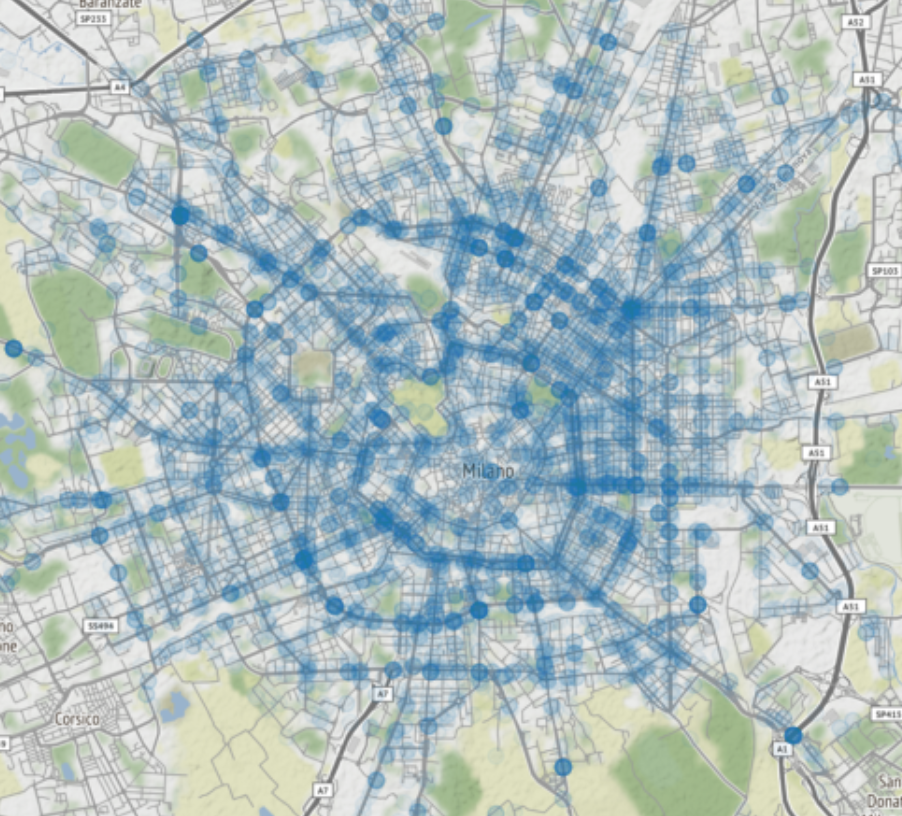
\includegraphics[width=\linewidth]{../src/incidenti/geo_incidenti.png}
    \caption{Distribuzione di incidenti a Milano}
    \label{fig:geo_incidenti}
\end{figure}

%...


\newpage
\section{Incidenti e Linee dei Trasporti Pubblici}

Il dataset dei tragitti dei trasporti pubblici copre molta pi\'u superficie rispetto a 
quello degli incidenti.
Dopo aver eliminato alcune linee di autobus che risultavano troppo in periferia, 
si nota comunque che i trasporti pubblici coprono la maggior parte di Milano.

\begin{figure}[!ht]
    \includegraphics[width=\linewidth]{../src/atm/mappa_2.png}
    \caption{Linee Autobus e Tram a Milano}
    \label{fig:geo_trasporti}
\end{figure}

Se a questi ultimi vengono sovrapposti i dati sugli incidenti, 
si pu\'o notare che la maggior parte dei luoghi con alta concentrazione di incidenti sono 
attraversati da linee di autobus. Nel caso di Corso Ventidue Marzo, si ha anche una linea di tram.


%...


Dalla sovrapposizione delle mappe, si pu\'o notare anche che, alcune strade con alta incidentalit\'a 
sono parallele a linee di autobus. Un esempio \'e quello di zona Navigli, 
dove le vie interessate sono:
Viale Gian Galeazzo e Viale Beatrice D'Este, parallele a Viale Col di Lana e Viale Bligny.
La stessa cosa si pu\'o notare su Viale Gabriele D'Annunzio e Viale Gorizia e Coni Zugna.

\begin{figure}[!ht]
    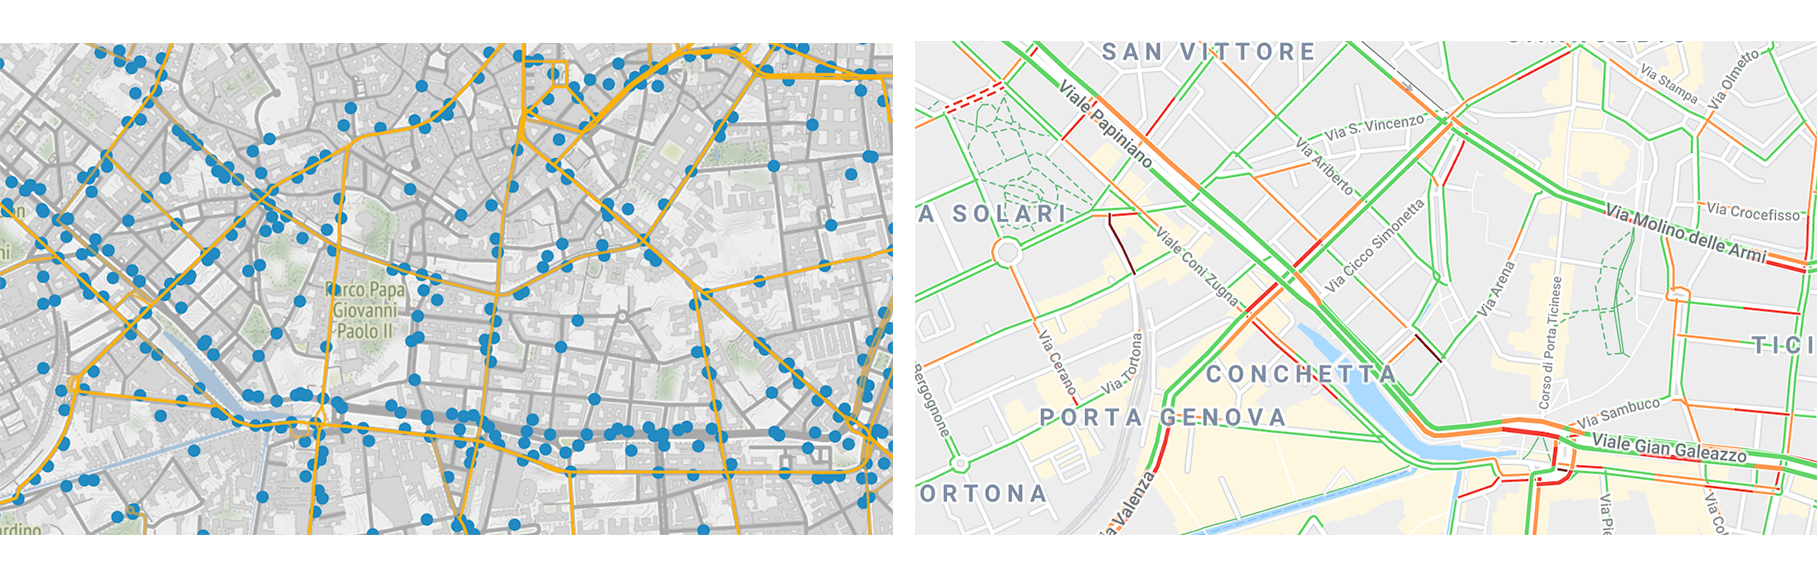
\includegraphics[width=\linewidth]{../src/atm/navigli.png}
    \caption{Linee Autobus e Tram a Milano}
    \label{fig:navigli}
\end{figure}

Anche vicino a corso Ventidue Marzo si pu\'o notare lo stesso fenomeno, 
tra Viale Bianca Maria e Viale Premuda.

\begin{figure}[!ht]
    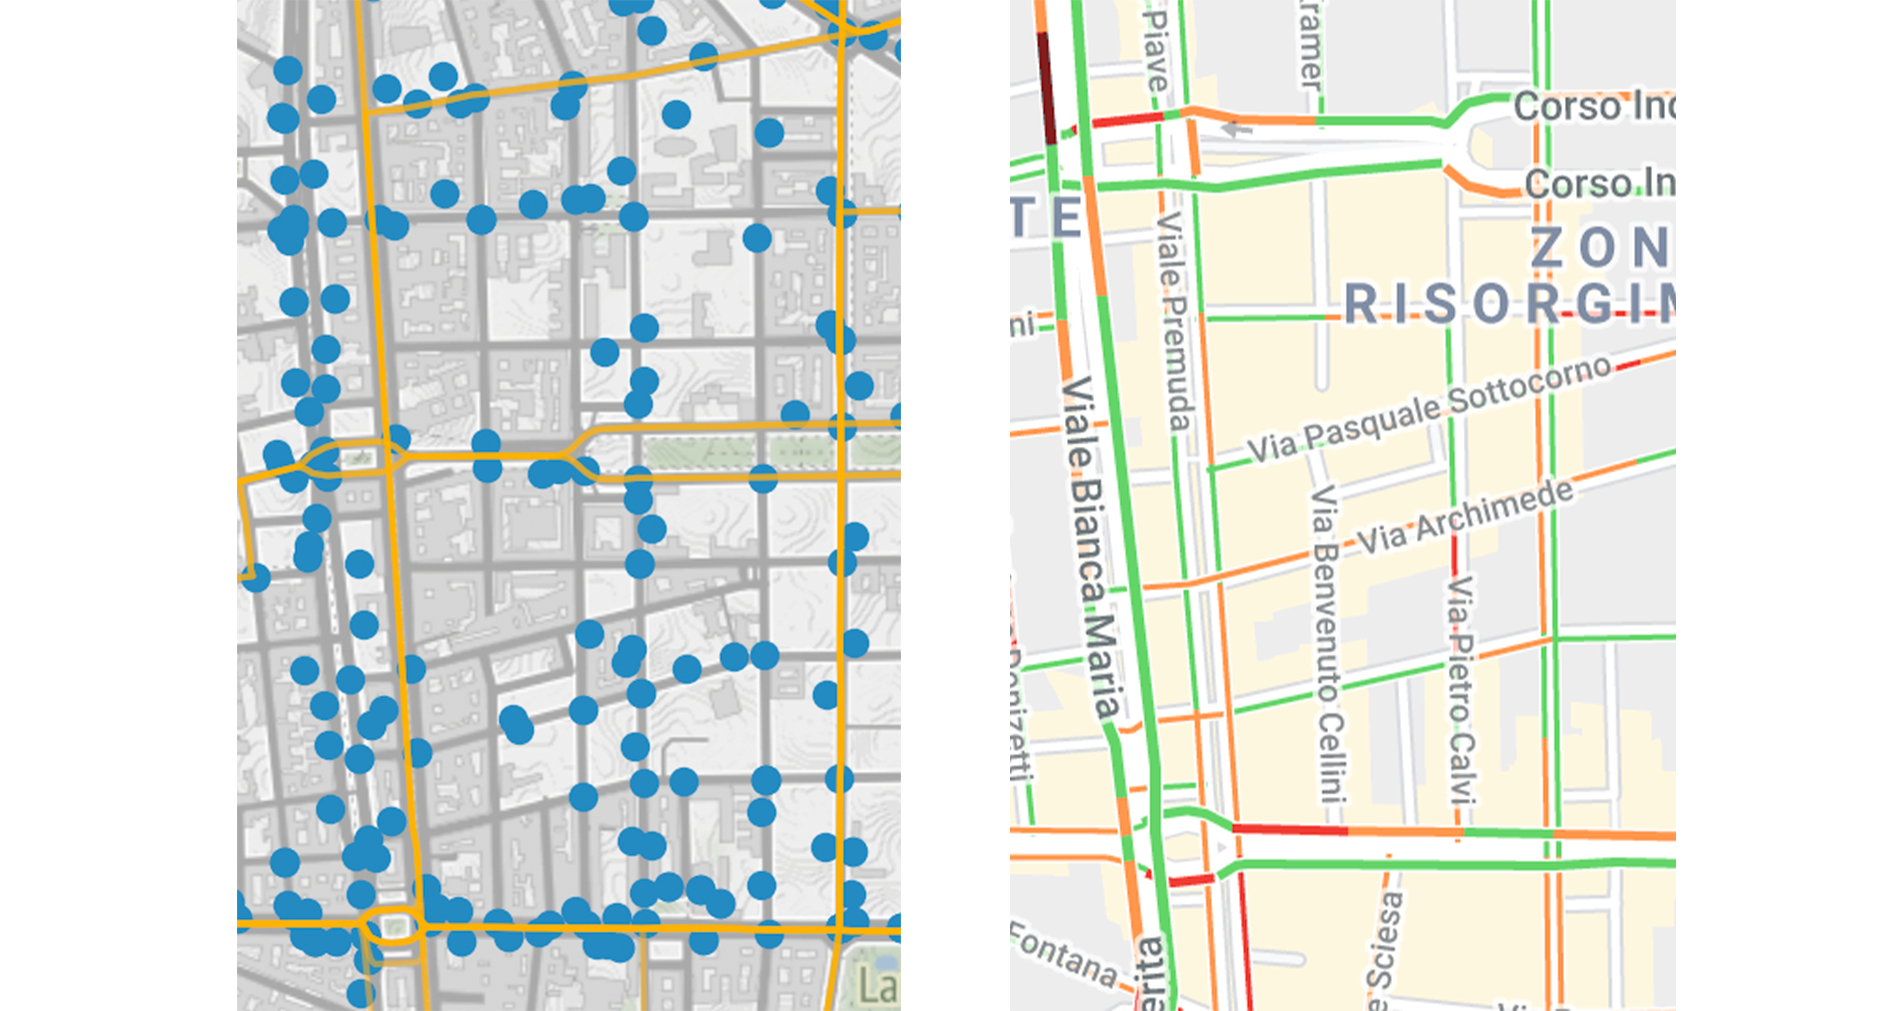
\includegraphics[width=\linewidth]{../src/atm/22_marzo.png}
    \caption{Linee Autobus e Tram a Milano}
    \label{fig:22_marzo}
\end{figure}

%...

\newpage
\subsection{Il Pav\'e influisce sull'incidentalit\'a?} Spesso le linee di tram coincidono con
strade in pav\'e
%...
Servirebbe una mappa delle strade in pave a Milano..

\newpage
\section{Incidenti e Piste  Ciclabili}

\newpage
\section{Incidenti e Autovelox}

Per sapere se gli autovelox hanno influenza sull'incidentalit\'a, 
bisognerebbe innanzi tutto sapere quando sono stati posizionati i dispositivi, e solo a quel punto, 
avendo dati su incidenti prima e dopo l'installazione, sarebbe possibile trarre conclusioni.

Alcuni dati sull'installazione di autovelox esistono per l'anno 2014, tuttavia i dati 
riguardo agli incidenti sono solo riguardanti l'anno 2016, in quanto Istat non ha rilasciato 
le posizioni degli incidenti in altre annate.

% TODO: devo scrivere come ho ricavato le posizioni degli autovelox installati nel 2014?
% (sono individuati tramite label) 


Gli autovelox installati nel 2014, presenti nel dataset, sono rappresentati nella seguente mappa.
\begin{figure}[!ht]
    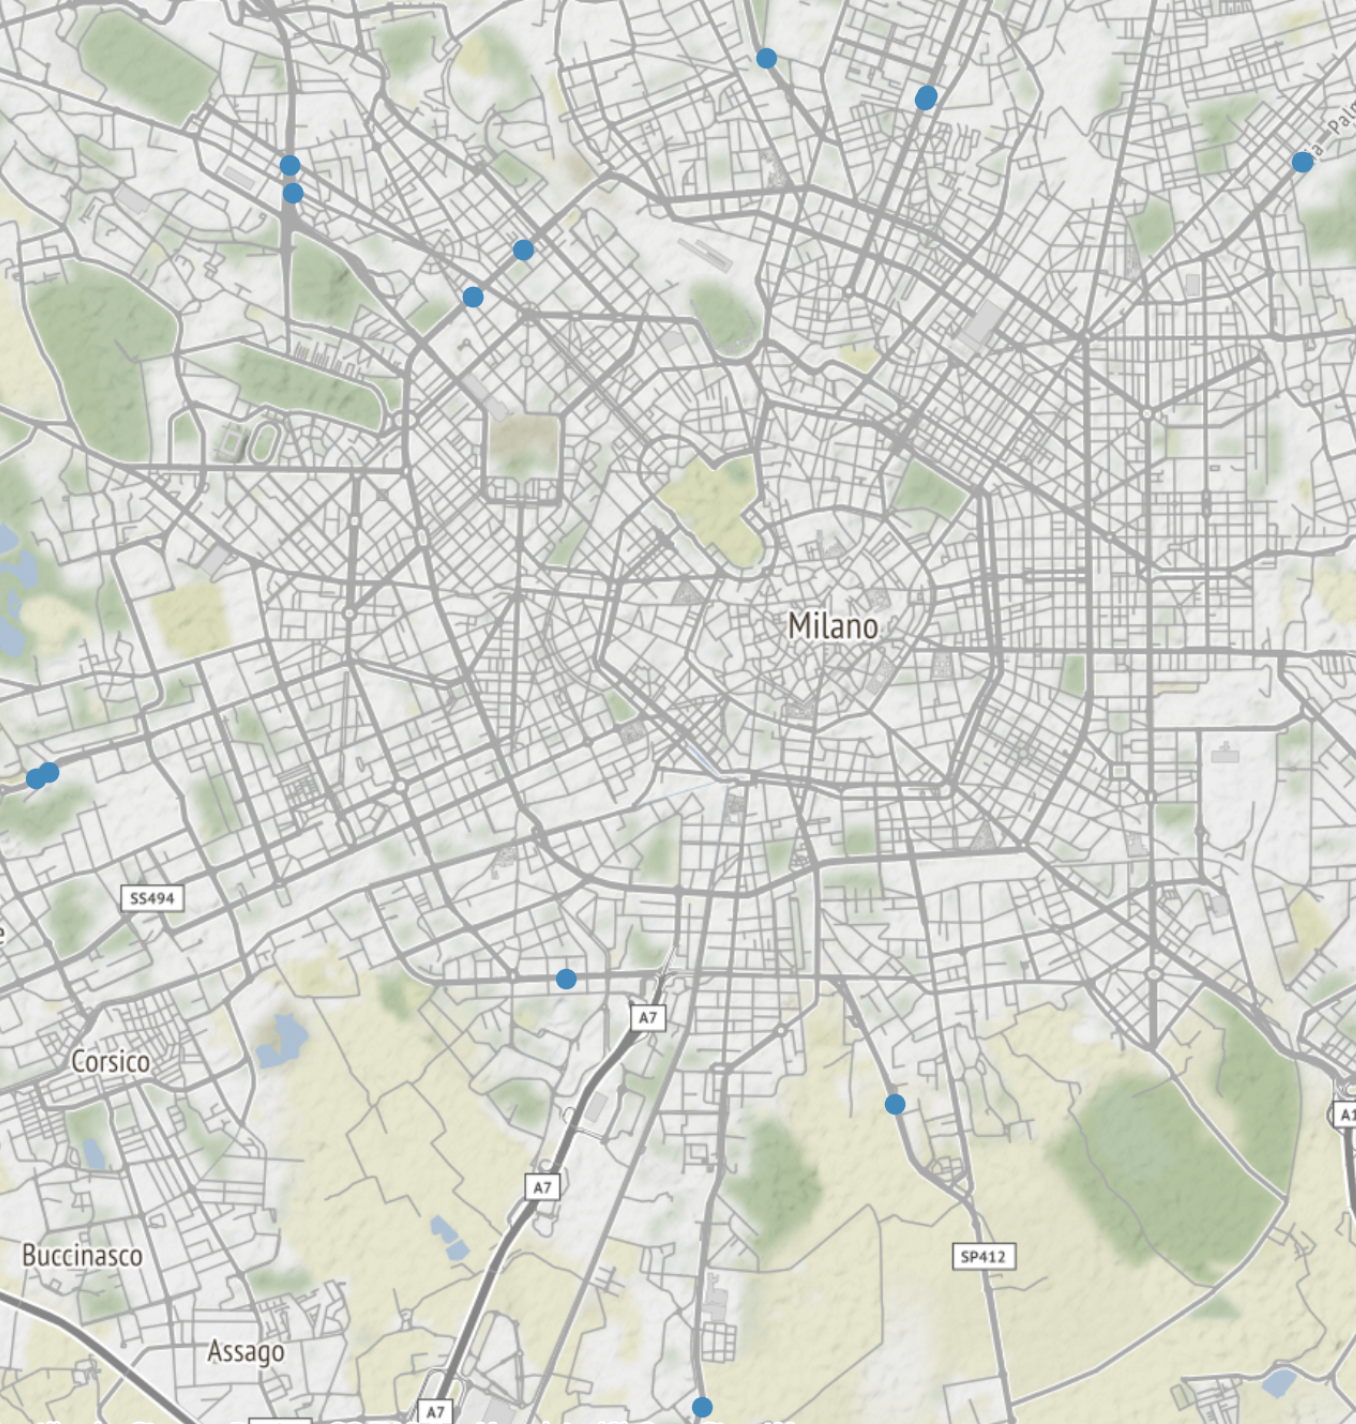
\includegraphics[width=\linewidth]{../src/autovelox/autovelox_2014.png}
    \caption{Autovelox installati nel 2014}
    \label{fig:autovelox_2014}
\end{figure}

\'E comunque possibile sovrapporre i dataset, per vedere se gli autovelox hanno un qualche tipo di 
effetto sugli incidenti.

\begin{figure}[!ht]
    \includegraphics[width=\linewidth]{../src/autovelox/mappa_3.png}
    \caption{Autovelox e Incidenti a Milano}
    \label{fig:autovelox}
\end{figure}

%...


\newpage
\section{Incidenti e Meteo}

%%%%%%%%%%%%%%%%%%%%%%%%%%%%%%%%%%%%%%%%%%%%%%%%%%%%%%
\newpage
\chapter{Dati su Incidenti}

Per quanto riguarda dati generali su incidenti in Italia, sono disponibili due dataset molto ampi, 
il primo, rilasciato da Istat, contiene dati dal 2010 al 2018 che riguardano campi come data, ora, 
numero di persone a bordo, tipo di incrocio, tipo di veicolo, ecc..
Il secondo \'e invece messo a disposizione da Automobile Club D'Italia (ACI) che contiene dati simili, 
ma in pi\'u mette a disposizione il luogo dell'incidente, come autostrada o strada provinciale.

\newpage
\section{Dati Istat su veicoli}

Il dataset Istat contiene molte informazioni riguardanti i conducenti dei veicoli coinvolti 
nell'incidente, oltre al tipo di veicoli.

\newpage
\subsection{Come cambia il tipo di veicolo al cambiare del tipo di strada?}

\begin{figure}[!ht]
    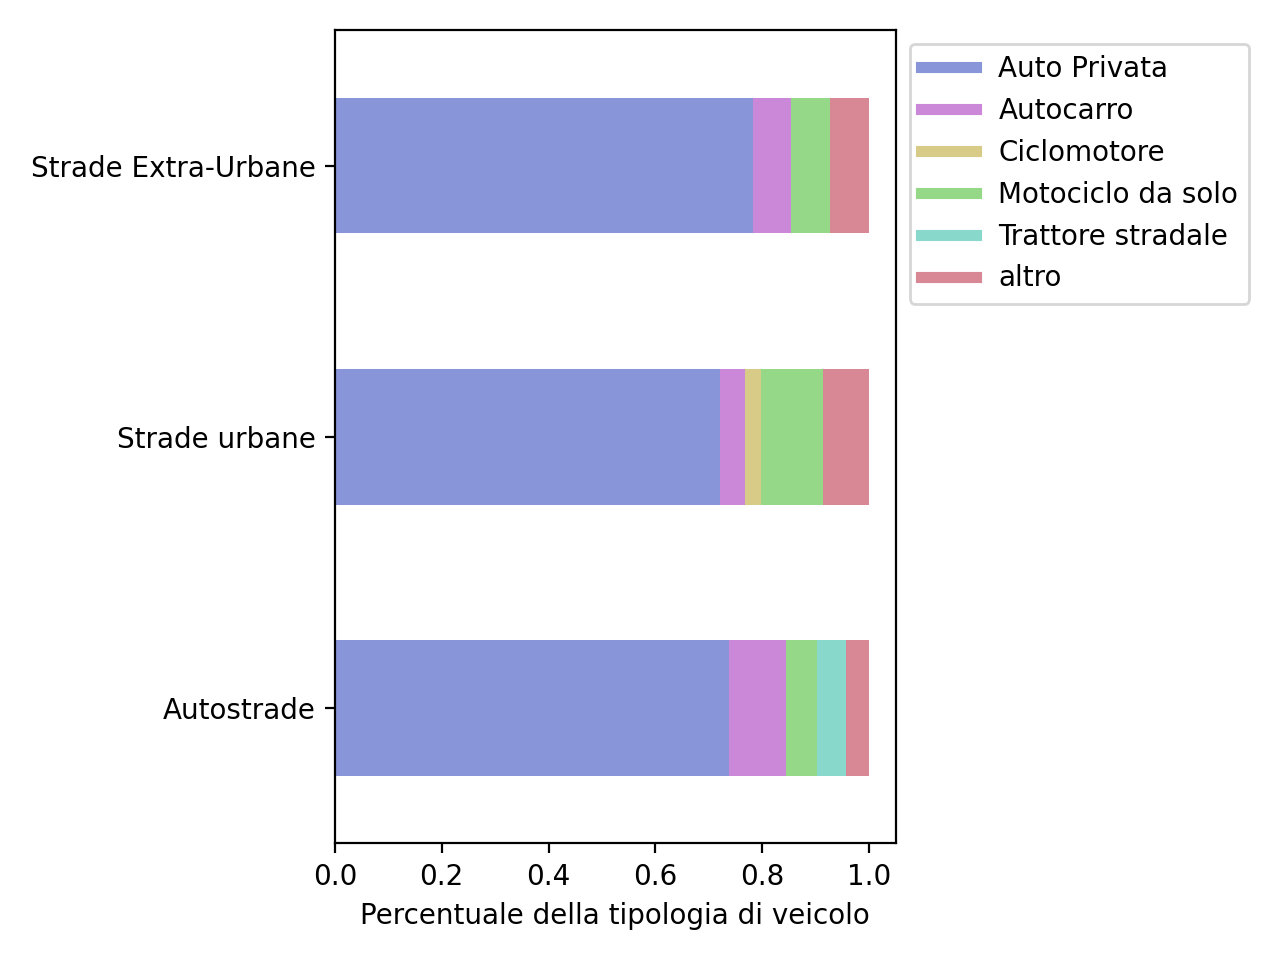
\includegraphics[width=\linewidth]{../src/incidenti/incidenti_senza_coords/tipo_veicoli/differenza_strade.png}
    \caption{Incidenti per tipo di veicolo nel 2010}
    \label{fig:differenza_strade}
\end{figure}

\'E possibile notare che, nonostante le auto private siano di gran lunga il tipo di veicolo 
pi\'u coinvolto in incidenti, nelle autostrade non sono presenti incidenti con velocipedi, 
anche il numero di incidenti con motocicli \'e ridotto, mentre cresce molto nelle strade urbane.


\newpage
\section{Dati Istat su conducente}

\newpage
\subsection{Come cambia il sesso del conducente al cambiare della strada?}

\begin{figure}[!ht]
    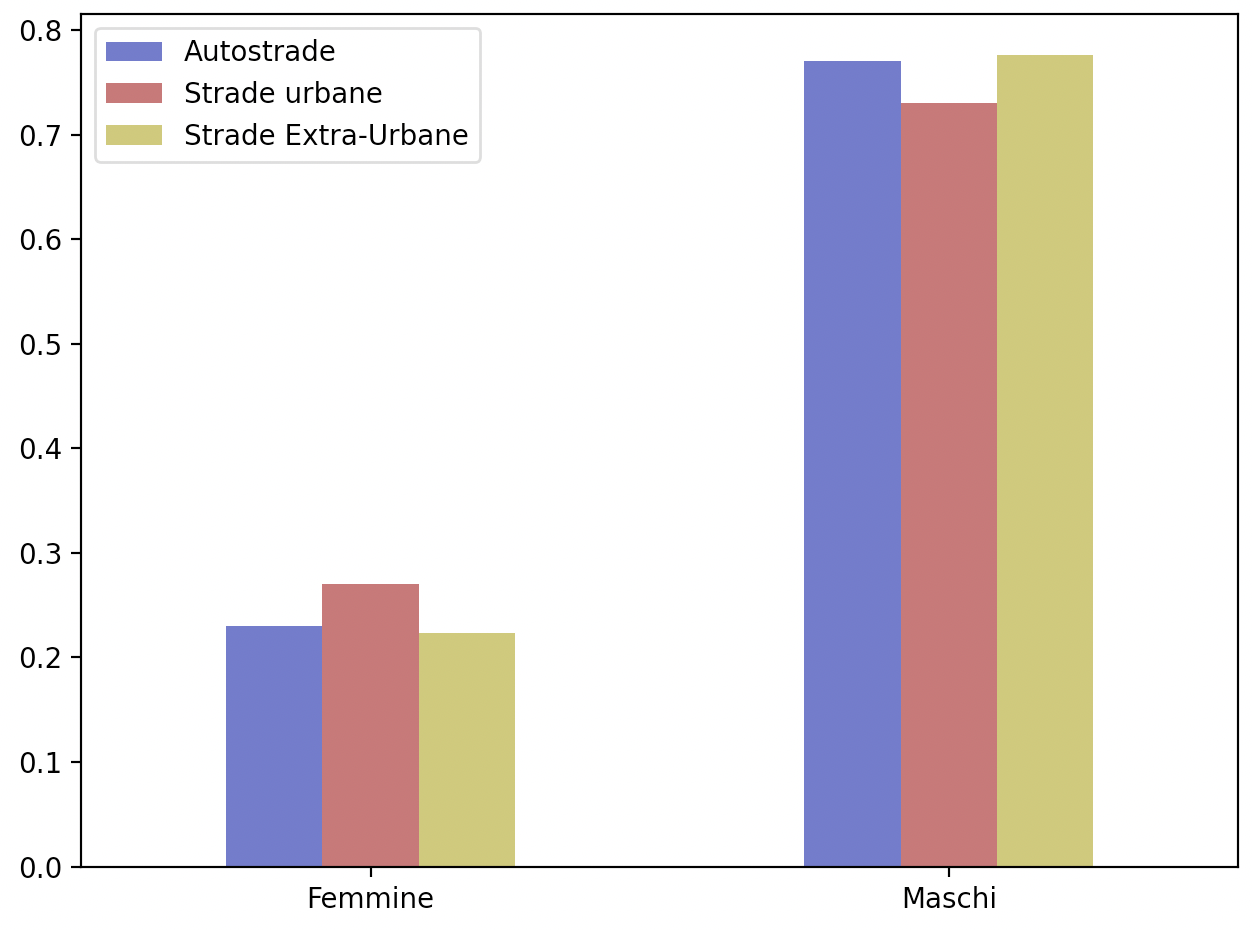
\includegraphics[width=\linewidth]{../src/incidenti/incidenti_senza_coords/tipo_veicoli/uomo-donna.png}
    \caption{Sesso del conducente per tipo di veicolo nel 2010}
    \label{fig:differenza_uomo_donna}
\end{figure}

Il numero di incidenti per genere \'e tende ad essere 75\% circa uomini e 25\% donne.
Nelle strade  urbane, la percentuale di incidenti con conducente donna aumenta leggermente nel 2010, 
questo vale per tutti gli anni?

%TODO: stima della percentuale di conducenti maschi/femmine


\newpage
\subsection{Come cambia l'et\'a del conducente al cambiare della strada?}

\begin{figure}[!ht]
    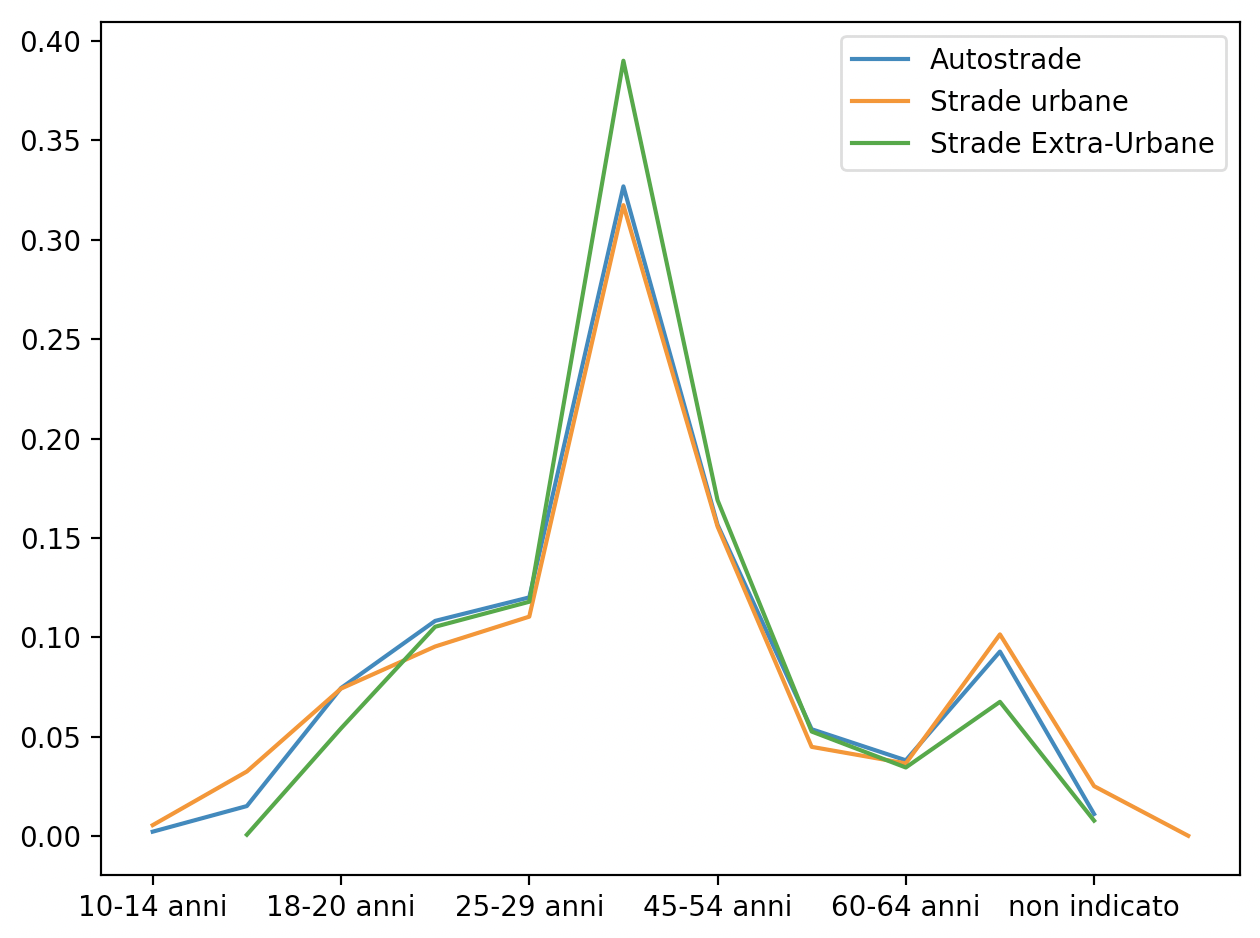
\includegraphics[width=\linewidth]{../src/incidenti/incidenti_senza_coords/tipo_veicoli/differenza_eta.png}
    \caption{Fascia di et\'a del conducente per tipo di veicolo nel 2010}
    \label{fig:differenza_eta}
\end{figure}

Risultati non troppo interessanti\dots

%...

\newpage
\subsection{Il numero di passeggeri influisce sull'incidentalit\'a?}

\begin{figure}[!ht]
    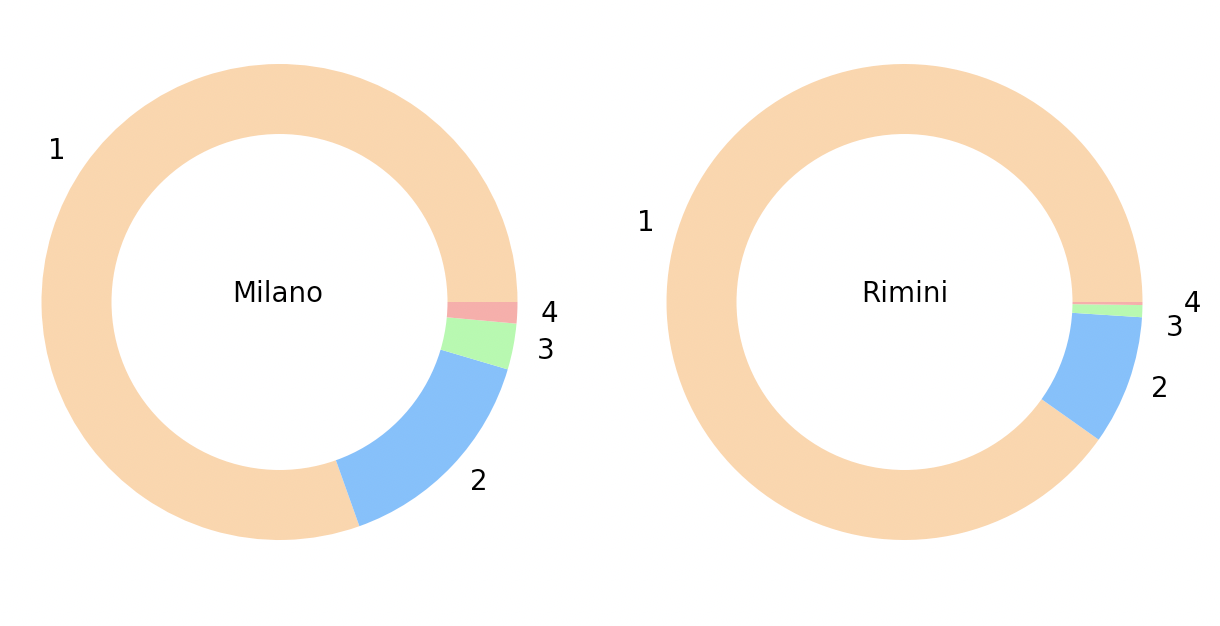
\includegraphics[width=\linewidth]{../src/incidenti/incidenti_senza_coords/tipo_veicoli/passeggeri.png}
    \caption{Numero di passeggeri in incidenti per Milano e Rimini}
    \label{fig:passeggeri_milano_rimini}
\end{figure}

La maggior parte degli incidenti sembra avvenire quando in macchina \'e presente solo il conducente.
Si sono prese in considerazione le provincie di Milano e Rimini, per controllare se la localit\'a 
marittima influisse sul numero di incidenti, ma sembra che quest'ultima abbia una percentuale 
ancora pi\'u alta di incidenti in cui \'e presente solo il conducente, rispetto a Milano.

\subsection{Il conducente se da solo si distrae con il telefono cellulare?}

Per quanto non siano disponibili dati su questo ambito, si potrebbe confrontare gli anni tra 2010 e 2013, 
in cui l'uso del cellulare in macchina ancora non era frequente, rispetto agli anni pi\'u recenti.

%...


\newpage
\section{Dati Istat su orari e mesi}

\newpage
\subsection{Quanto influiscono le ore di punta sull'incidentalit\'a?}

Per prima cosa, con un semplice conto degli incidenti durante il weekend 
e confrontandolo con il numero di quelli avvenuti durante la 
settimana lavorativa, si osserva che nel weekend avvengon pi\'u incidenti 
durante la sera e la notte, mentre durante la settimana in giornata.

\begin{figure}[!ht]
    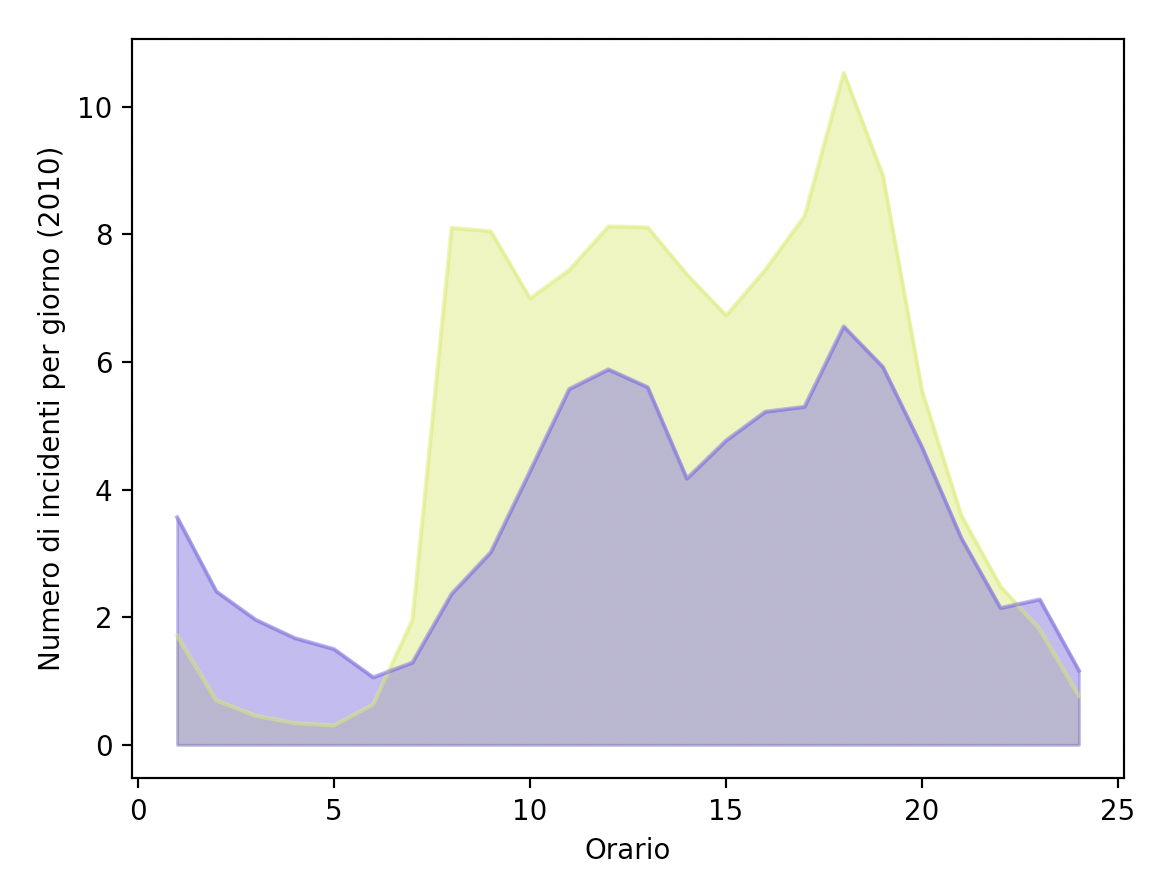
\includegraphics[width=\linewidth]{../src/incidenti/incidenti_senza_coords/ore_punta/week_weekend.png}
    \caption{Incidenti per ora}
    \label{fig:week_weekend}
\end{figure}

Per quanto riguarda gli orari di punta, 
sono state prese in considerazione due fasce orarie, la prima, 
mattutina dalle 7:00 alle 10:00, e la seconda pomeridiana, 
dalle 17:00 alle 19:00

\begin{figure}
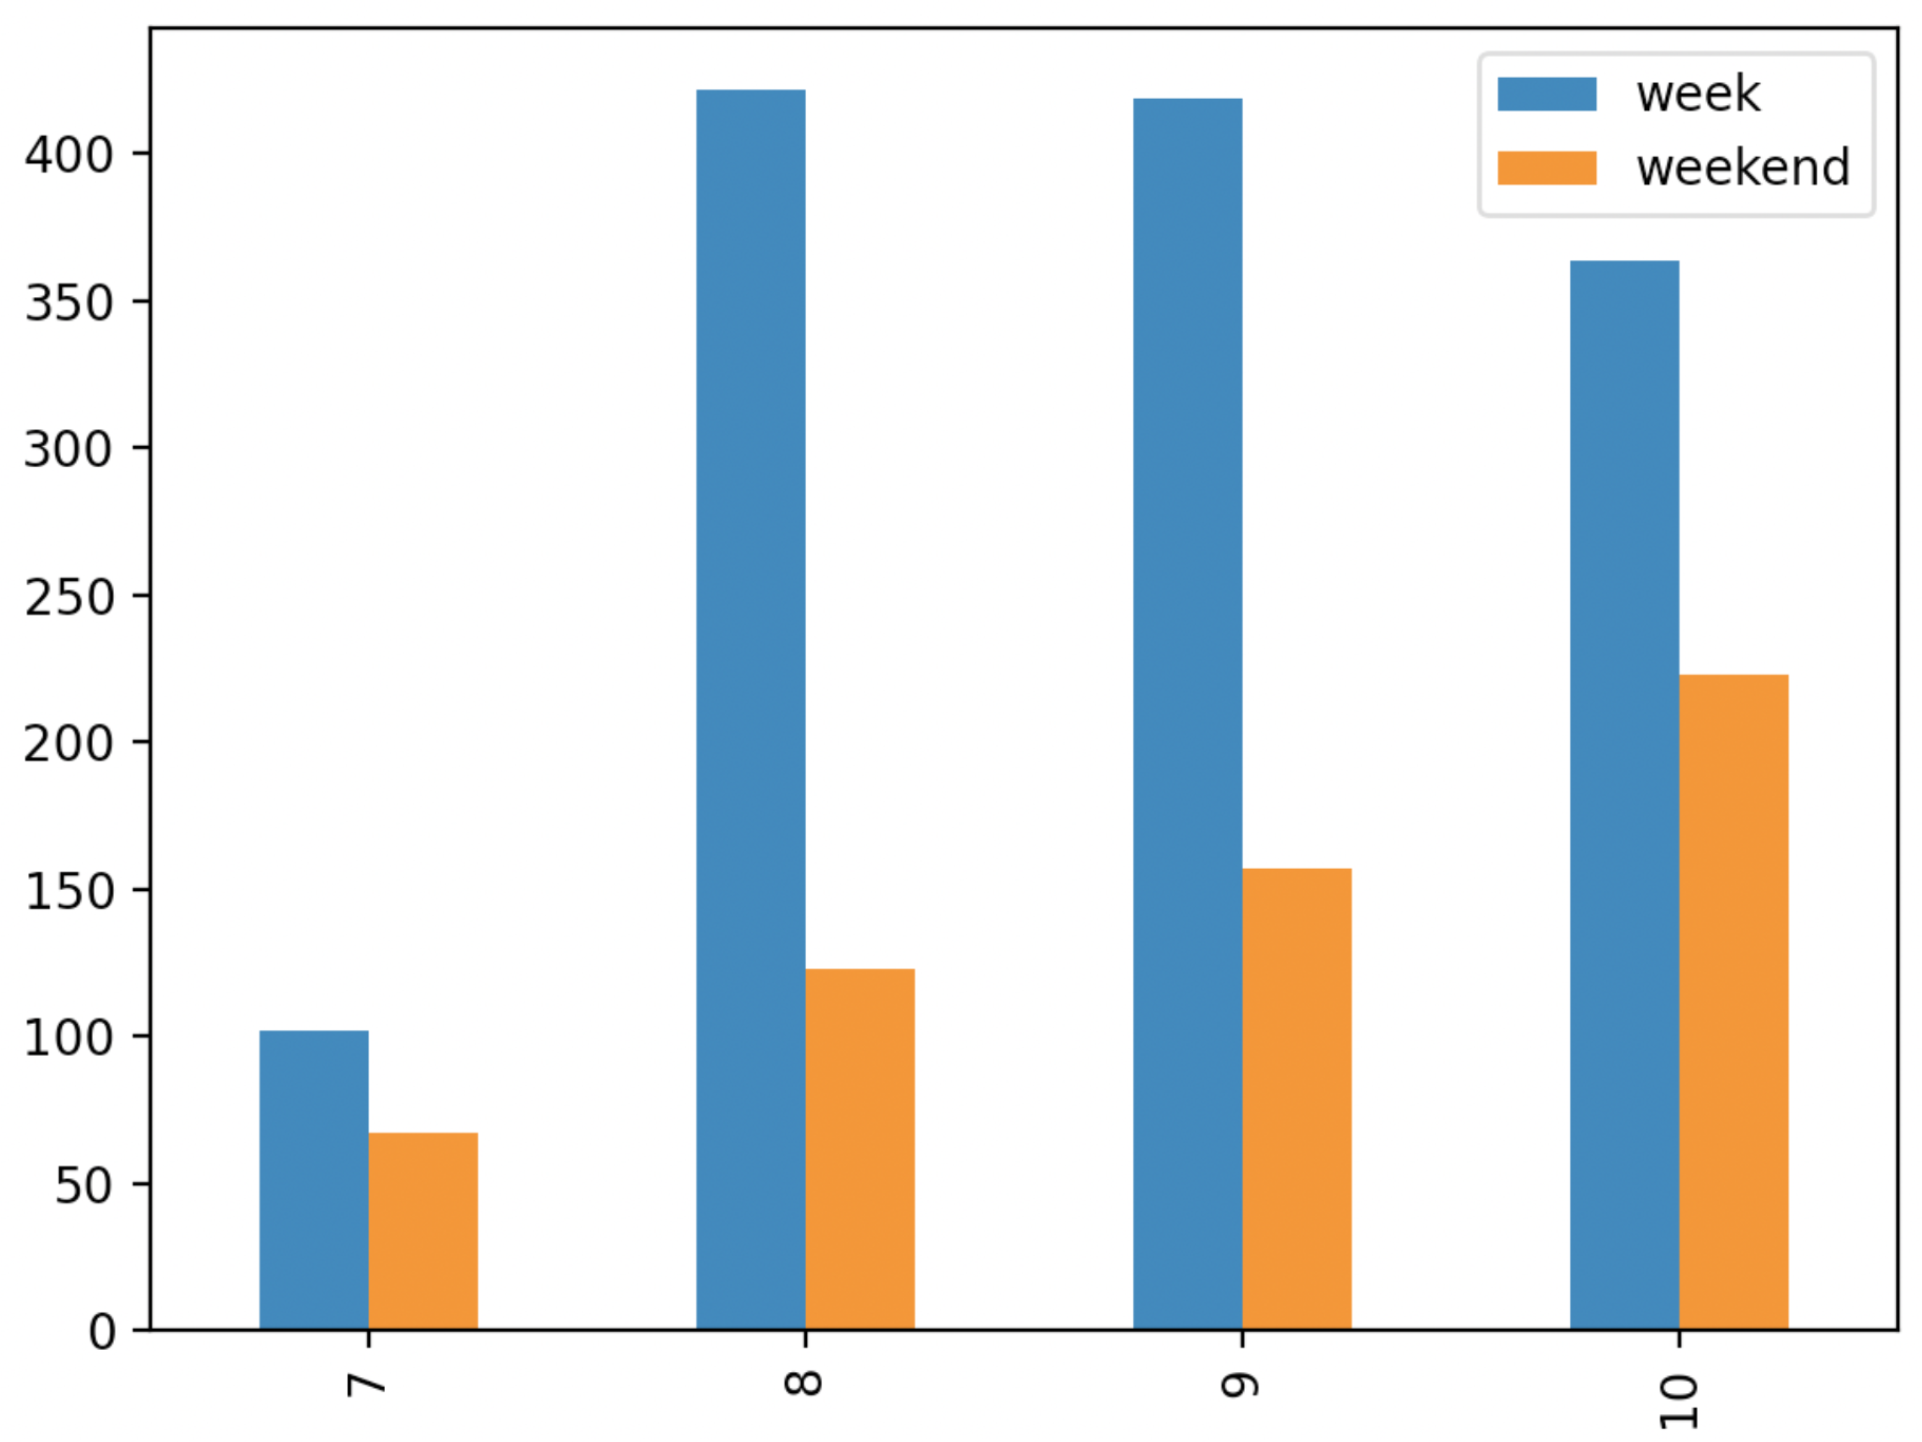
\includegraphics[width=\linewidth]{../src/incidenti/incidenti_senza_coords/ore_punta/ore_punta_mattina.png}
\caption{Ore di punta Mattutine}
\label{fig:punta_mattina}
\end{figure}

\begin{figure}
    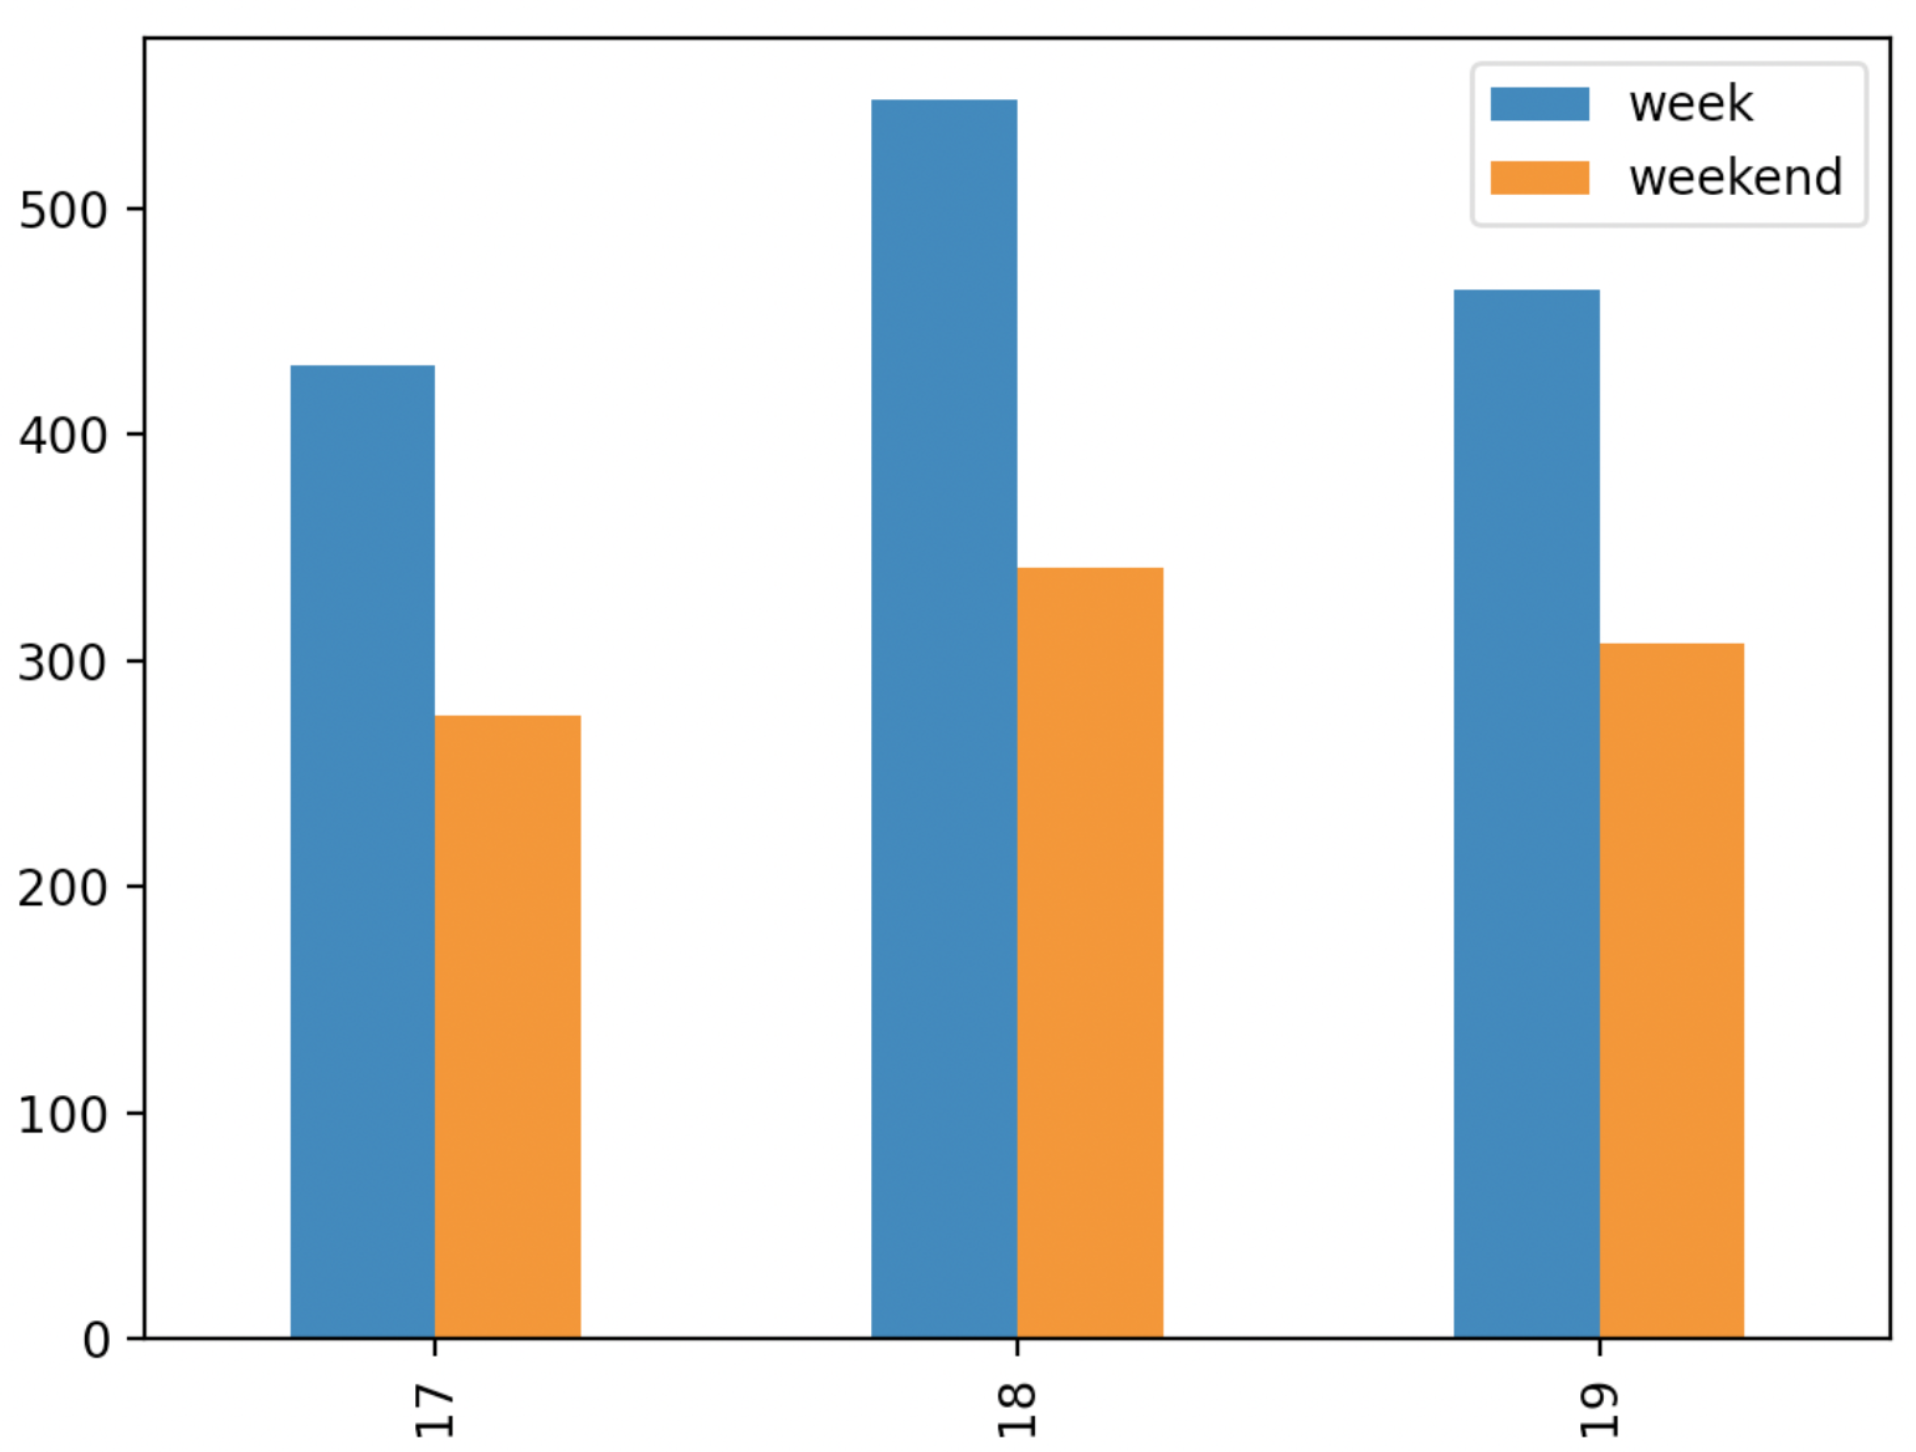
\includegraphics[width=\linewidth]{../src/incidenti/incidenti_senza_coords/ore_punta/ore_punta_sera.png}
    \caption{Ore di punta serali}
    \label{fig:punta_sera}
\end{figure}


Va sottolineato che i grafi indicano gli incidenti normalizzati per numero di 
giorni, 
quindi gli incidenti totali della settimana sono divisi per cinque giorni, 
mentre quelli del weekend per due.
Si pu\'o osservare che nella fascia oraria delle 18:00, 
avvengono molti pi\'u sinistri, mentre nella fascia mattutina, 
il numero non sembra variare molto dalla media di incidenti durante il giorno.

\newpage
\subsection{\'E possibile accentuare le ore di punta mattutine?}

Se si selezionano solo gli incidenti nella provincia di Milano, \'e possibile individuare 
il secondo picco di incidenti, quello durante le ore di punta mattutine

\begin{figure}[!ht]
    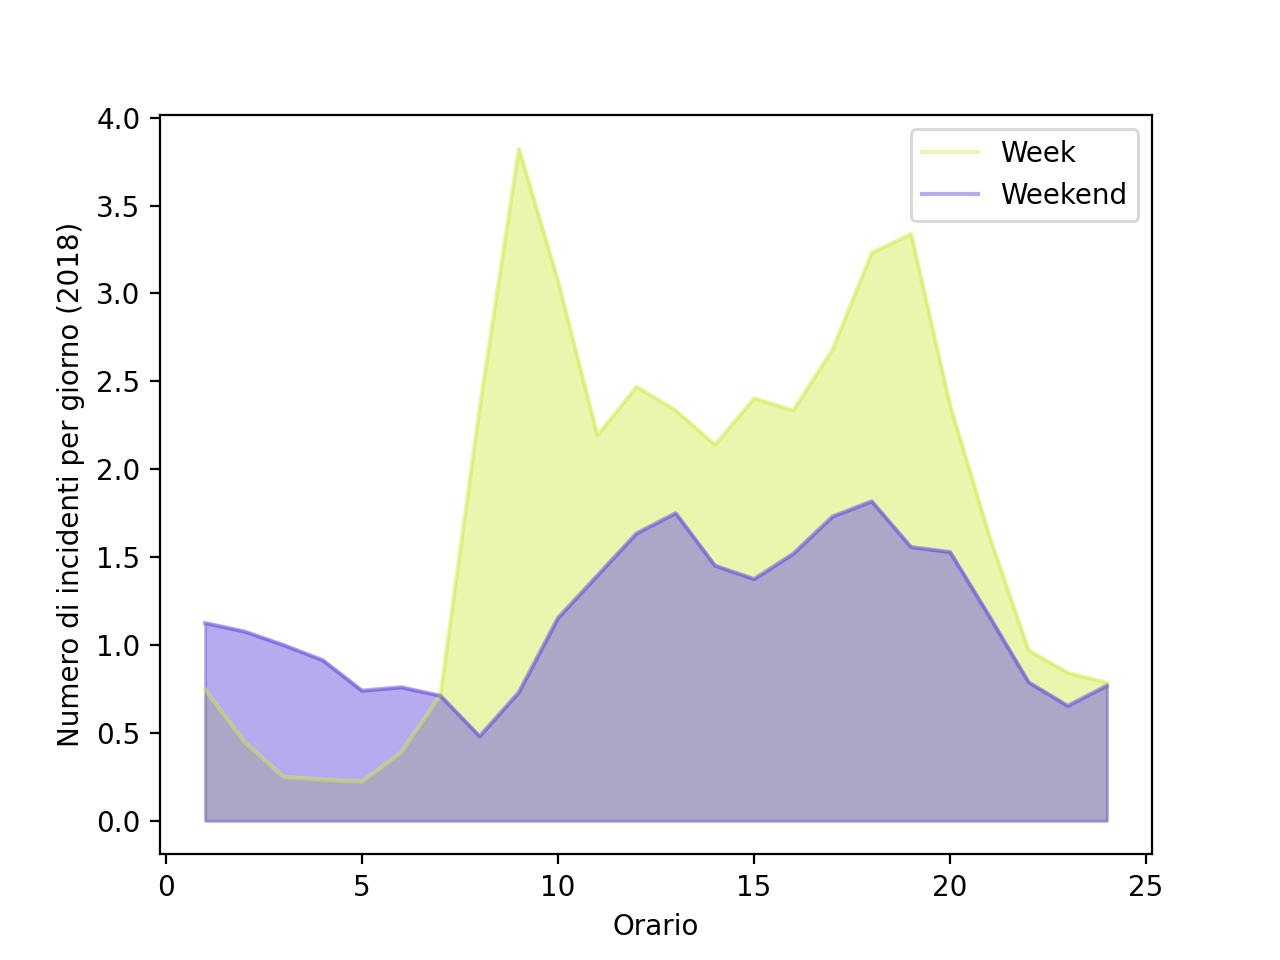
\includegraphics[width=\linewidth]{../src/incidenti/incidenti_senza_coords/ore_punta/week_weekend_milano.png}
    \caption{Incidenti per ora a Milano}
    \label{fig:week_weekend_milano}
\end{figure}

%...

\newpage
\subsection{Si ha la stessa tendenza di notte?}

Come individuato dal primo grafo in \label{fig:week_weekend}, durante le 
ore notturne si ha la tendenza opposta.

\begin{figure}[!ht]
    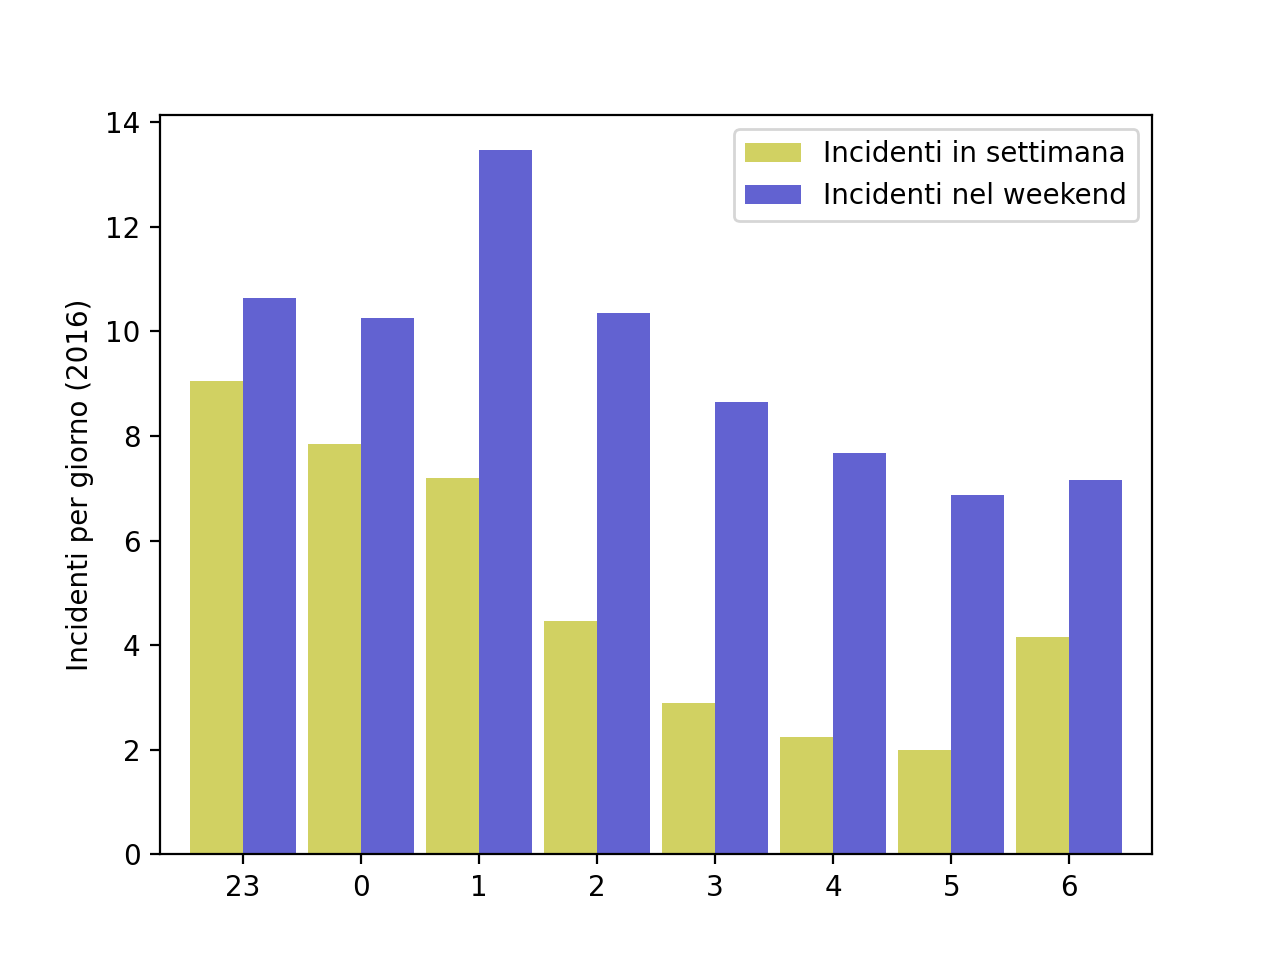
\includegraphics[width=\linewidth]{../src/incidenti/incidenti_senza_coords/ore_punta/ore_notte.png}
    \caption{Incidenti durante ore serali o notturne}
    \label{fig:ore_notte}
\end{figure}

%...

\newpage
\subsection{Quanto influiscono le vacanze estive sull'incidentalit\'a?}

\begin{figure}[!ht]
    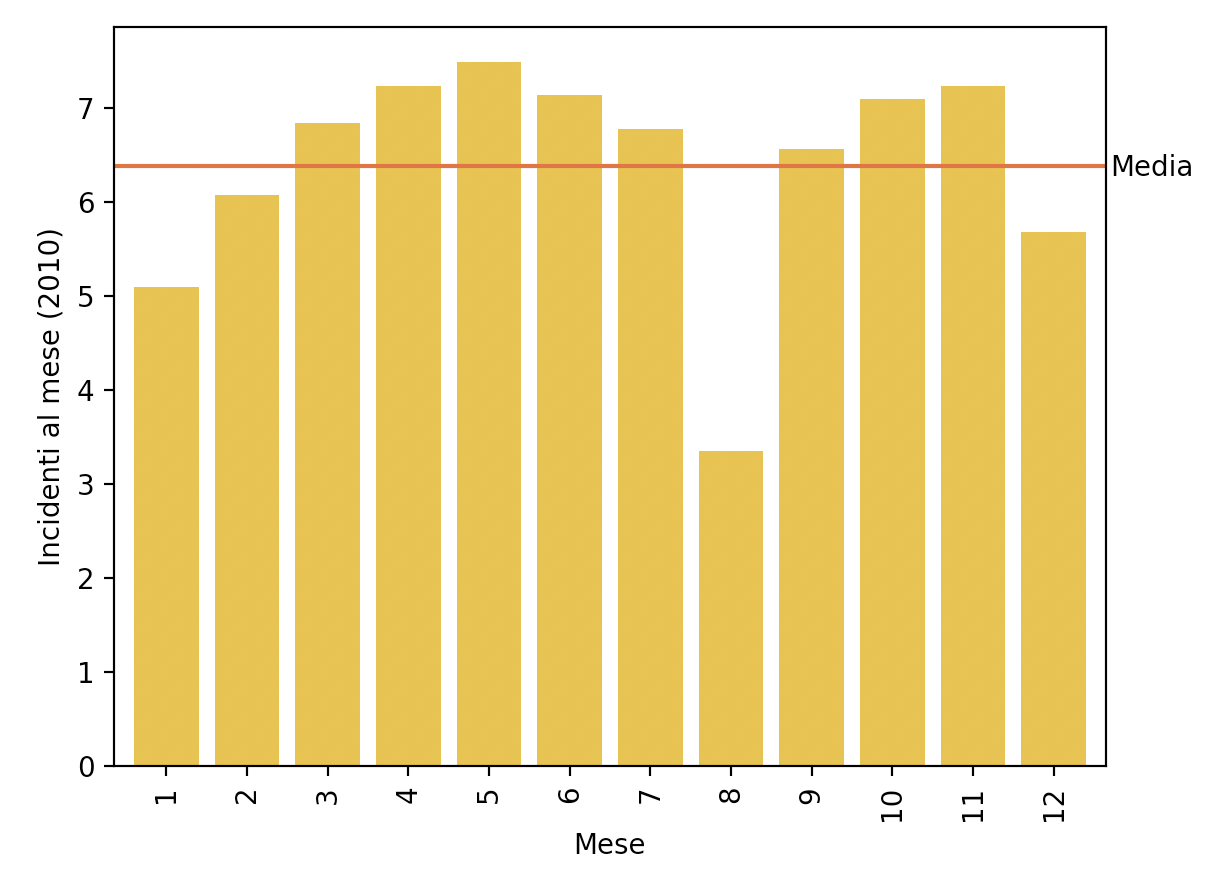
\includegraphics[width=\linewidth]{../src/incidenti/incidenti_senza_coords/mese_incidenti/milano_mese.png}
    \caption{Incidenti per mese in Milano}
    \label{fig:milano_mese}
\end{figure}

Si nota un chiaro calo di incidenti nel mese di Agosto in provincia di Milano.
Per quanto possano esserci molti fattori che contribuiscono a questa tendenza, 
quello che influisce di pi\'u devono essere le partenze per le vacanze.

\newpage
\subsection{\'E possibile individuare la tendenza inversa in localit\'a  di mare?}

\begin{figure}[!ht]
    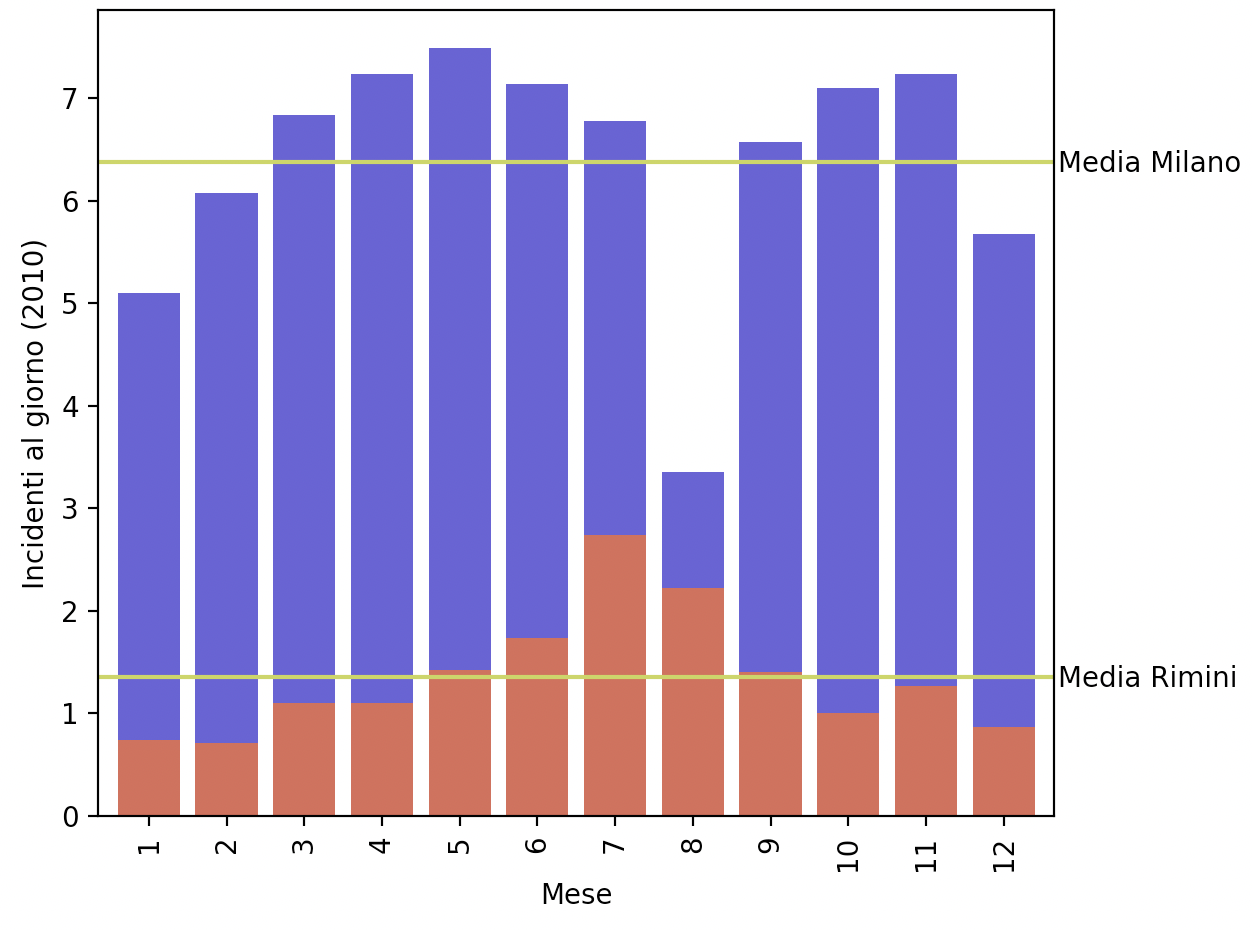
\includegraphics[width=\linewidth]{../src/incidenti/incidenti_senza_coords/mese_incidenti/milano_rimini.png}
    \caption{Incidenti per mese in Milano e Rimini}
    \label{fig:milano_rimini}
\end{figure}

L'unica localit\'a in cui si \'e riscontrata la tendenza inversa \'e in provincia 
di Rimini.
Tuttavia, osservando il grafo equivalente della Valle d'Aosta, \'e possibile notare 
un notevole incremento di incidenti sia in Gennaio che in Agosto, possibili 
conseguenze, rispettivamente, dell'inizio della stagione sciistica ed estiva.

\begin{figure}[!ht]
    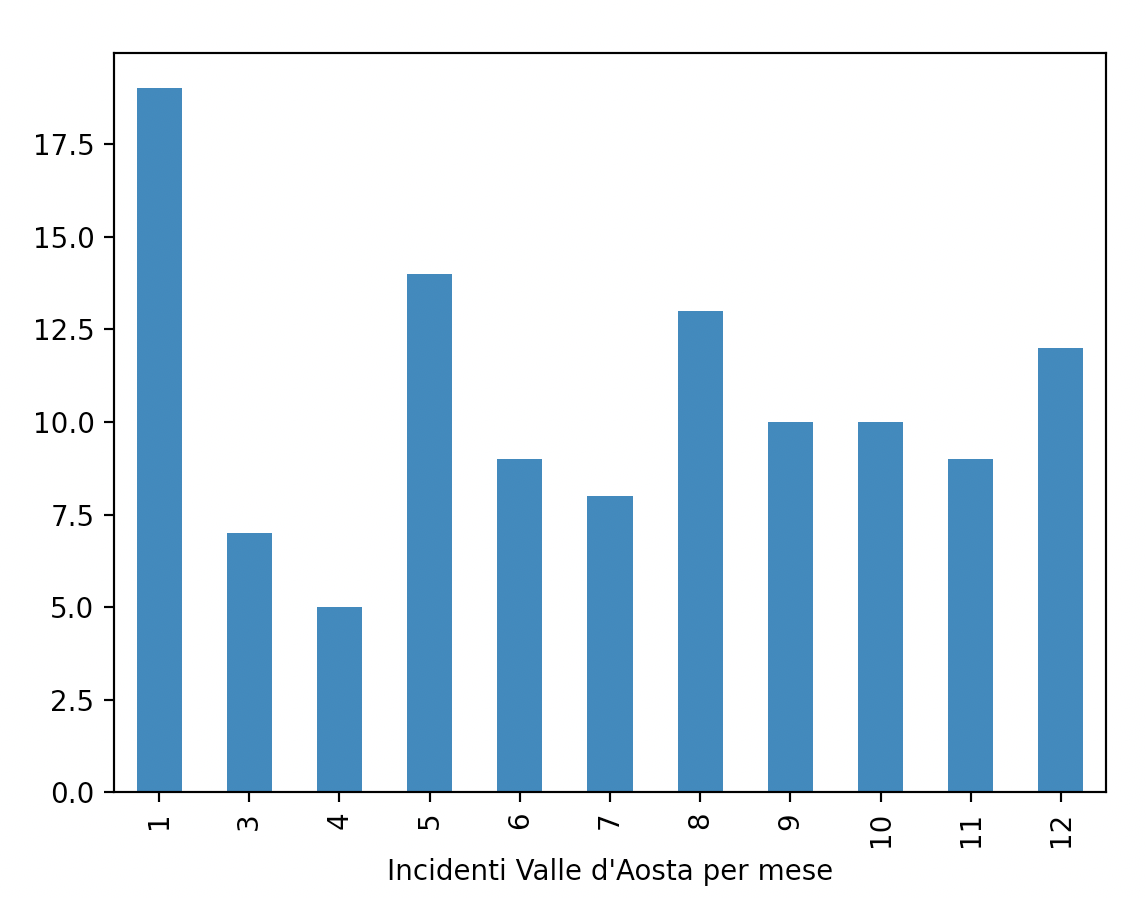
\includegraphics[width=\linewidth]{../src/incidenti/incidenti_senza_coords/mese_incidenti/valle_aosta.png}
    \caption{Incidenti per mese Valle d'Aosta}
    \label{fig:aosta}
\end{figure}

Questa tendenza avviene ogni anno?
Negli anni successivi al 2013 il campo 'mese' viene sostituito da 'trimestre', 
dunque nei i grafi seguenti gli indici non indicano pi\'u i mesi.

\begin{figure}[!ht]
    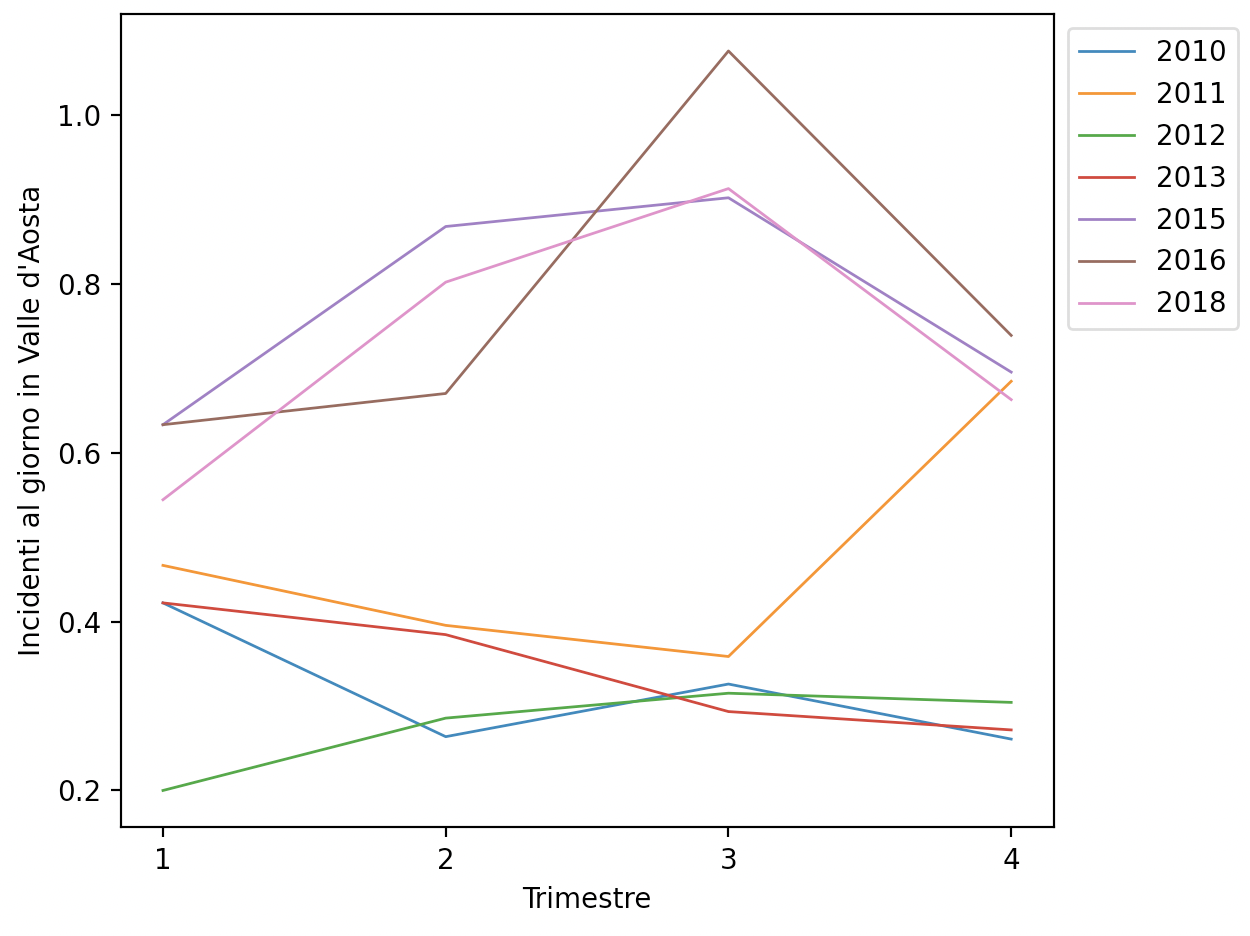
\includegraphics[width=\linewidth]{../src/incidenti/incidenti_senza_coords/mese_incidenti/aosta_timestre.png}
    \caption{Incidenti per trimestre in Valle d'Aosta}
    \label{fig:aosta_trimestre}
\end{figure}

La prima cosa che \'e possibile notare, \'e che il picco di Gennaio del 2010 \'e 
in linea con la tendenza del trimestre invernale. 
Tuttavia, si osserva anche che dall'anno 2015 c'\'e un ampio gap nel numero di 
incidenti. 
\'E un cambio di metro di misurazione? 

\begin{figure}[!ht]
    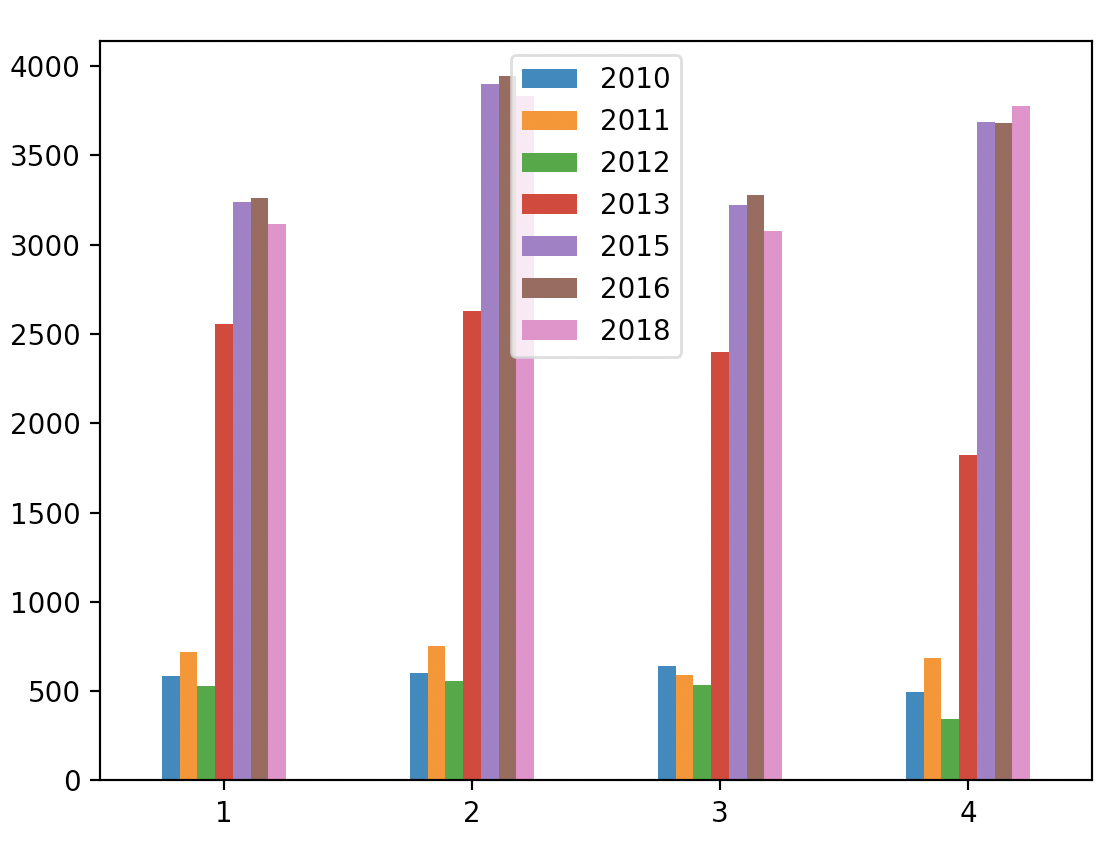
\includegraphics[width=\linewidth]{../src/incidenti/incidenti_senza_coords/mese_incidenti/milano_trimestre.png}
    \caption{Incidenti per trimestre a Milano}
    \label{fig:milano_trimestre}
\end{figure}

\begin{figure}[!ht]
    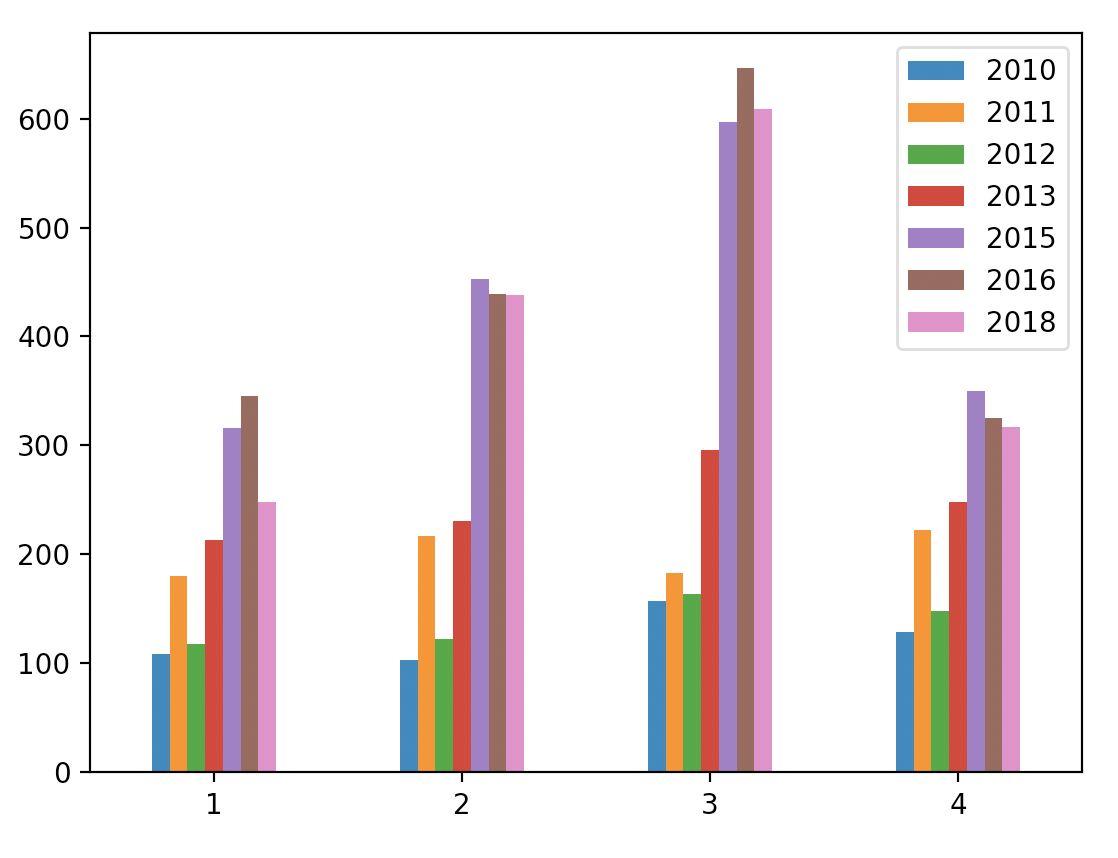
\includegraphics[width=\linewidth]{../src/incidenti/incidenti_senza_coords/mese_incidenti/rimini_trimestre.png}
    \caption{Incidenti per trimestre a Rimini}
    \label{fig:rimini_trimestre}
\end{figure}

I grafi equivalenti di Milano e Rimini mostrano la stessa tendenza di incremento del numero 
di incidenti, ma a Milano, in particolare, il gap sembra essersi 'creato' nel 2013.

%...

\newpage
\section{Dati Istat su tipi di incidenti e incroci}

\newpage
\subsection{Quali incidenti avvengono con pi\'u frequenza?}

\begin{figure}[!ht]
    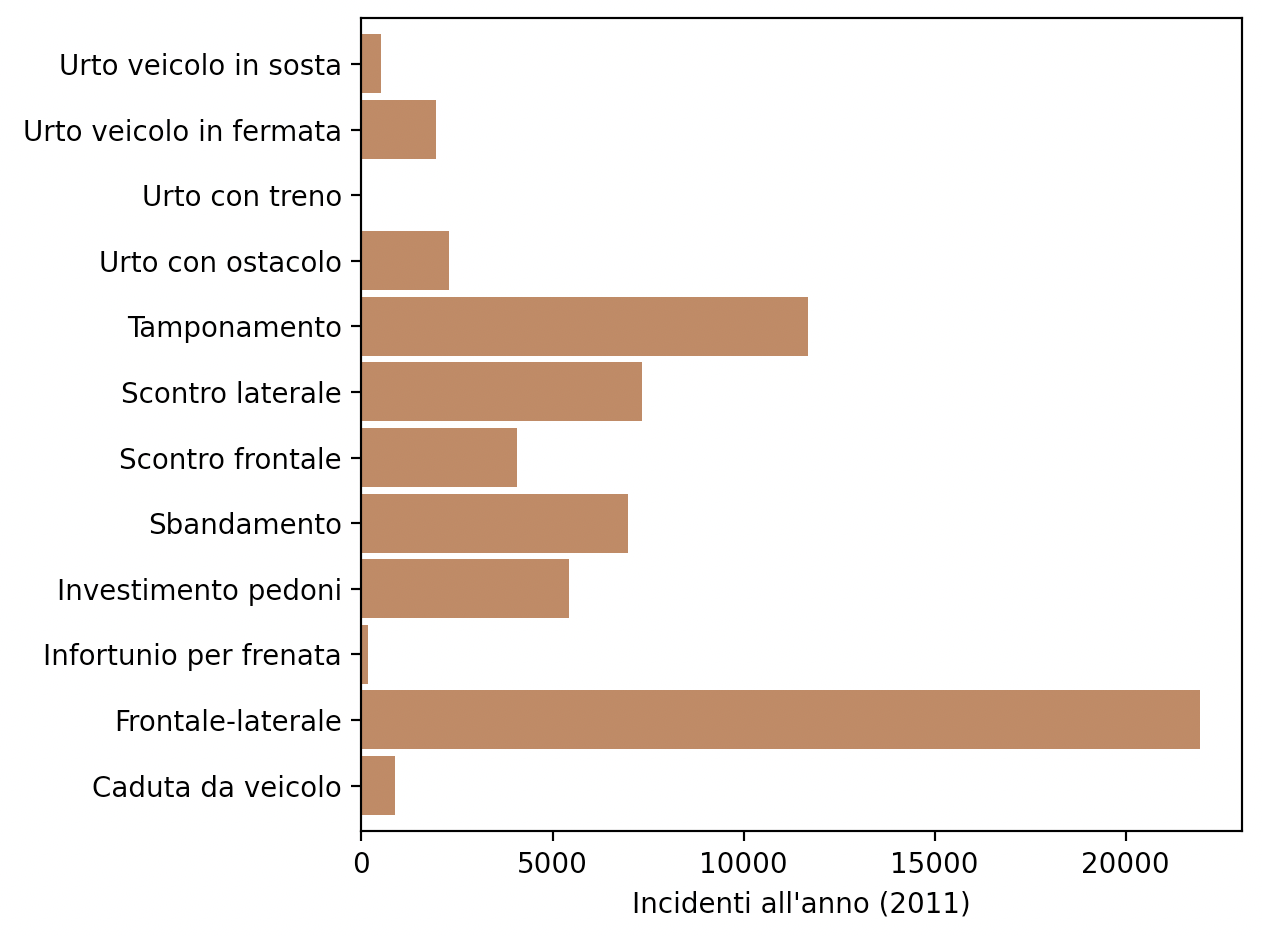
\includegraphics[width=\linewidth]{../src/incidenti/incidenti_senza_coords/localizzazione_incidente/tipo_incidente.png}
    \caption{Tipologia di incidente}
    \label{fig:tipo_incidente}
\end{figure}

Sono molto frequenti scontri frontali, laterali e tamponamenti.

\newpage
\subsection{Quali tipi di incroci provocano pi\'u incidenti?}

\begin{figure}[!ht]
    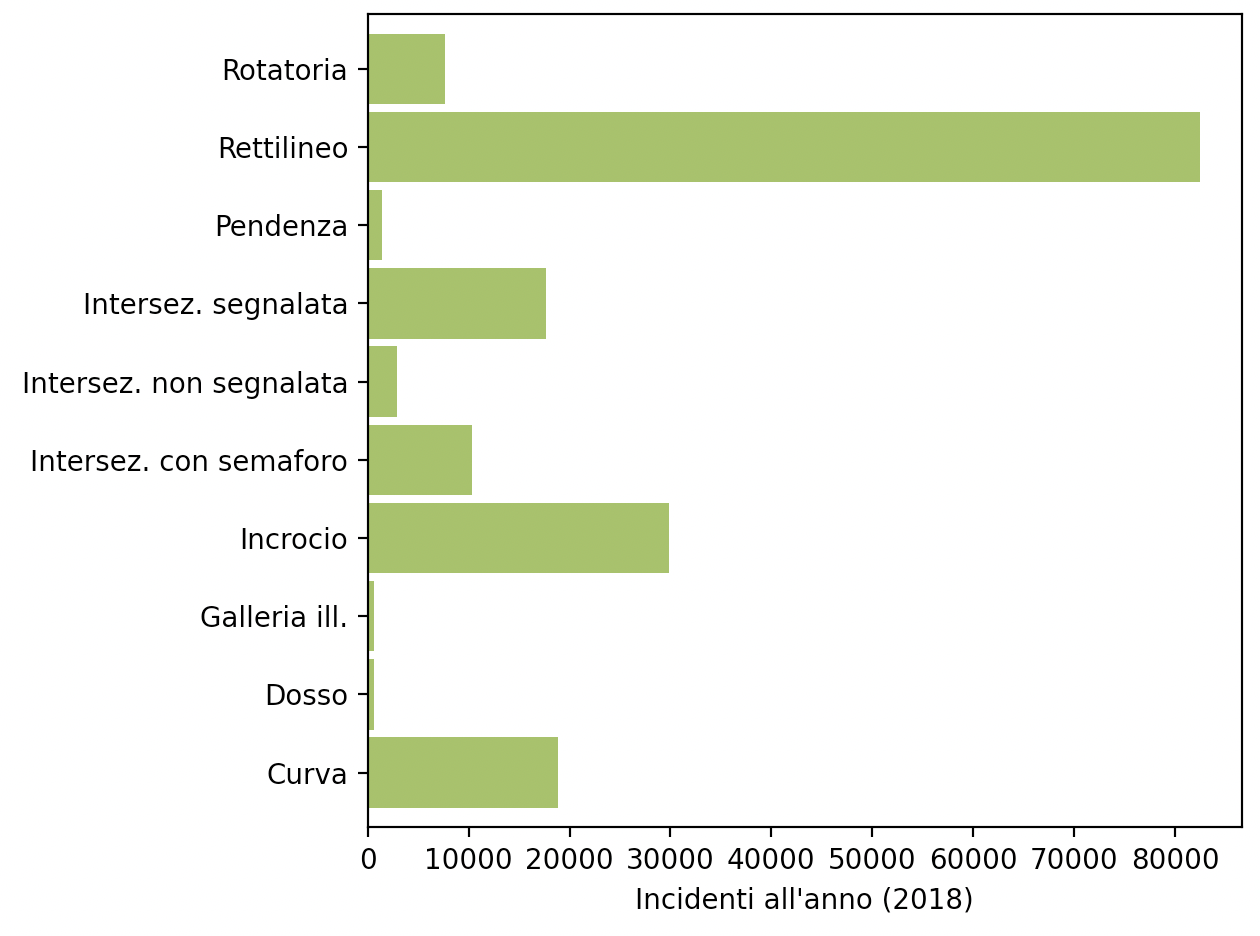
\includegraphics[width=\linewidth]{../src/incidenti/incidenti_senza_coords/localizzazione_incidente/intersezioni.png}
    \caption{Tipologia di intersezioni}
    \label{fig:tipo_intersezioni}
\end{figure}

La maggior parte degli incidenti avviene nei rettilinei e negli incroci.

%...

\newpage
\subsection{Esistono incroci che favoriscono incidenti con pedoni?}

\begin{figure}[!ht]
    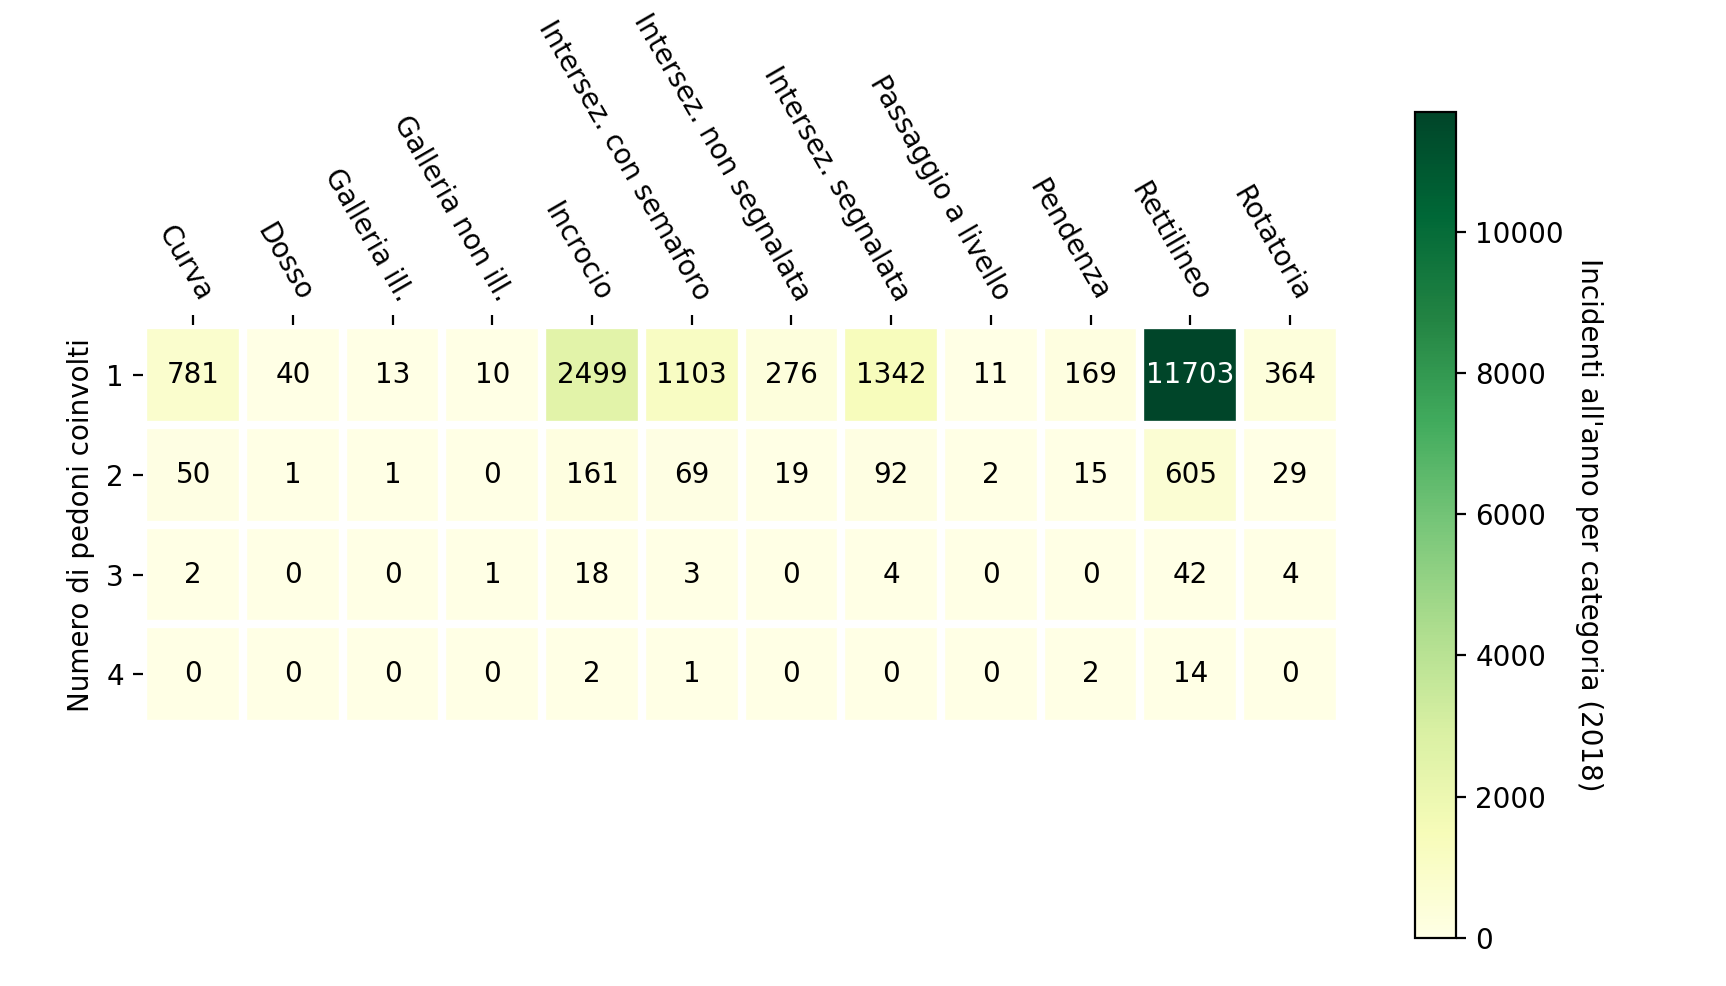
\includegraphics[width=\linewidth]{../src/incidenti/incidenti_senza_coords/pedoni/pedoni_incroci.png}
    \caption{Tipologia di intersezioni e pedoni coinvolti}
    \label{fig:pedoni_intersezioni}
\end{figure}

Tra i tipi di strada che favoriscono incidenti con pedoni spiccano i rettilinei, 
probabilmente in parte per l'alta velocit\'a dei veicoli, ma anche per l'alto volume di
tratti di strada di questo tipo.

%...

\newpage
\subsection{Ci sono caratteristiche interessanti dei pedoni coinvolti?}

\begin{figure}[!ht]
    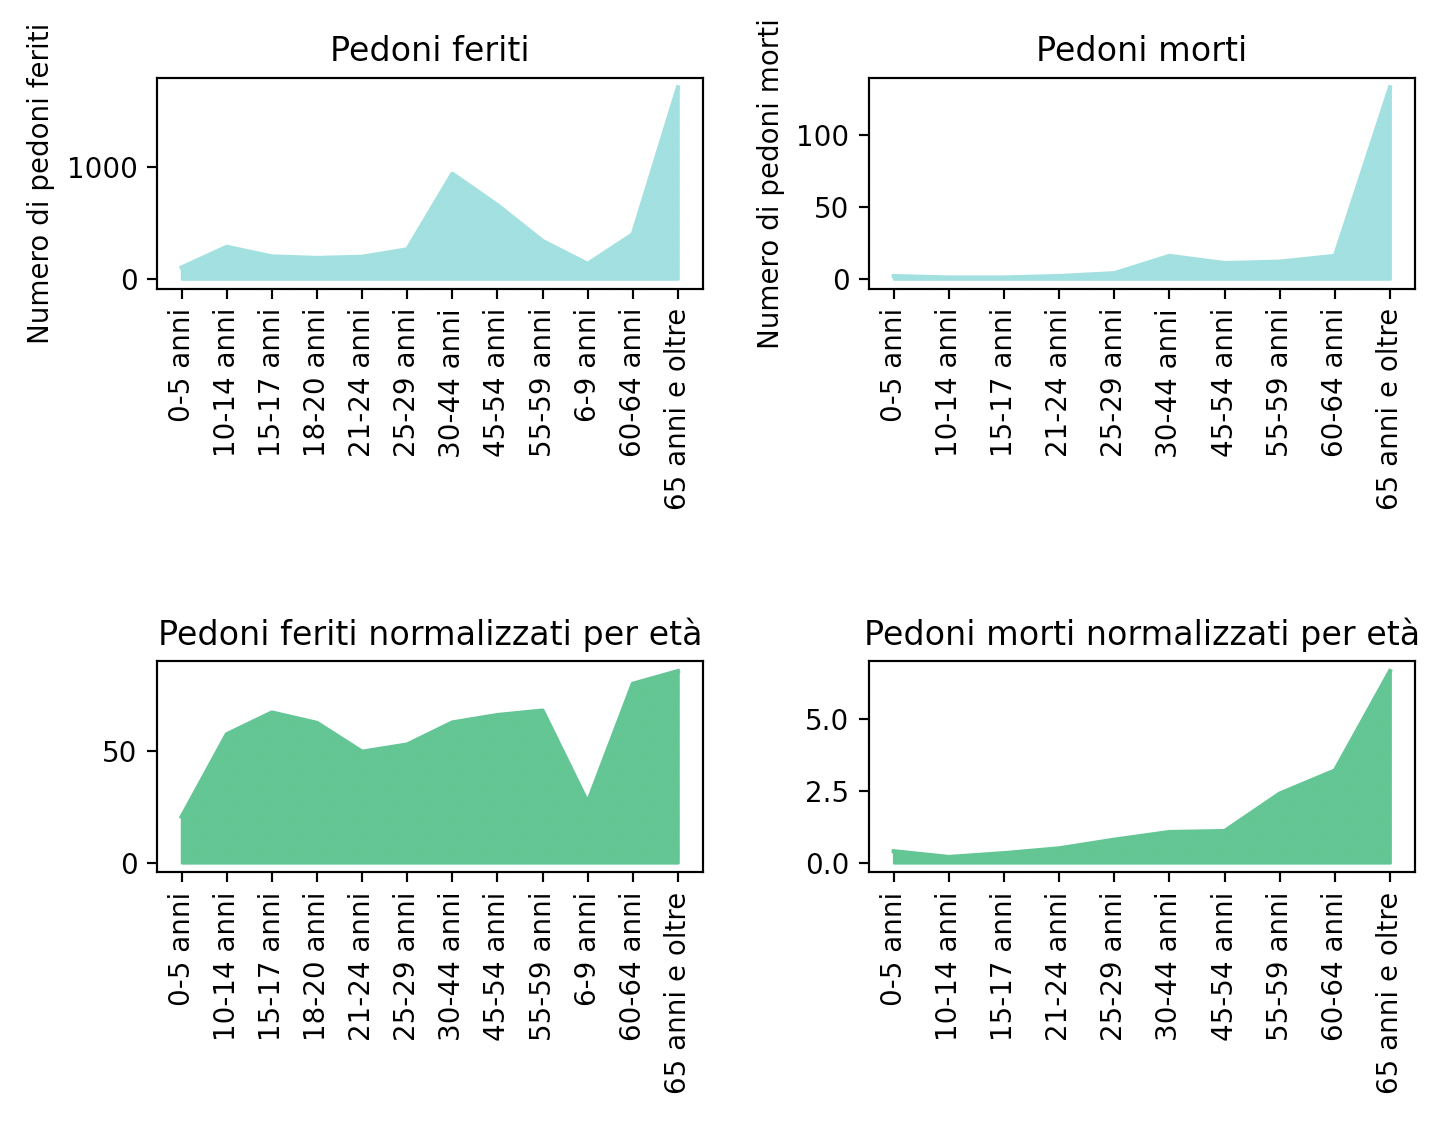
\includegraphics[width=\linewidth]{../src/incidenti/incidenti_senza_coords/pedoni/eta_pedoni.png}
    \caption{Fasce di et\'a dei pedoni coinvolti in incidenti}
    \label{fig:eta_pedoni}
\end{figure}

La fascia di et\'a pi\'u colpita dagli incidenti \'e quella dei 65 anni, 
va comunque detto che questo gruppo probabilmente contiene la maggior parte degli individui.
Se si normalizza per anni contenuti in ogni fascia, ipotizzando un numero
costante di persone di ogni et\'a, si ottiene un grafo, per quanto riguarda i pedoni 
feriti, molto differente. 

\begin{figure}[!ht]
    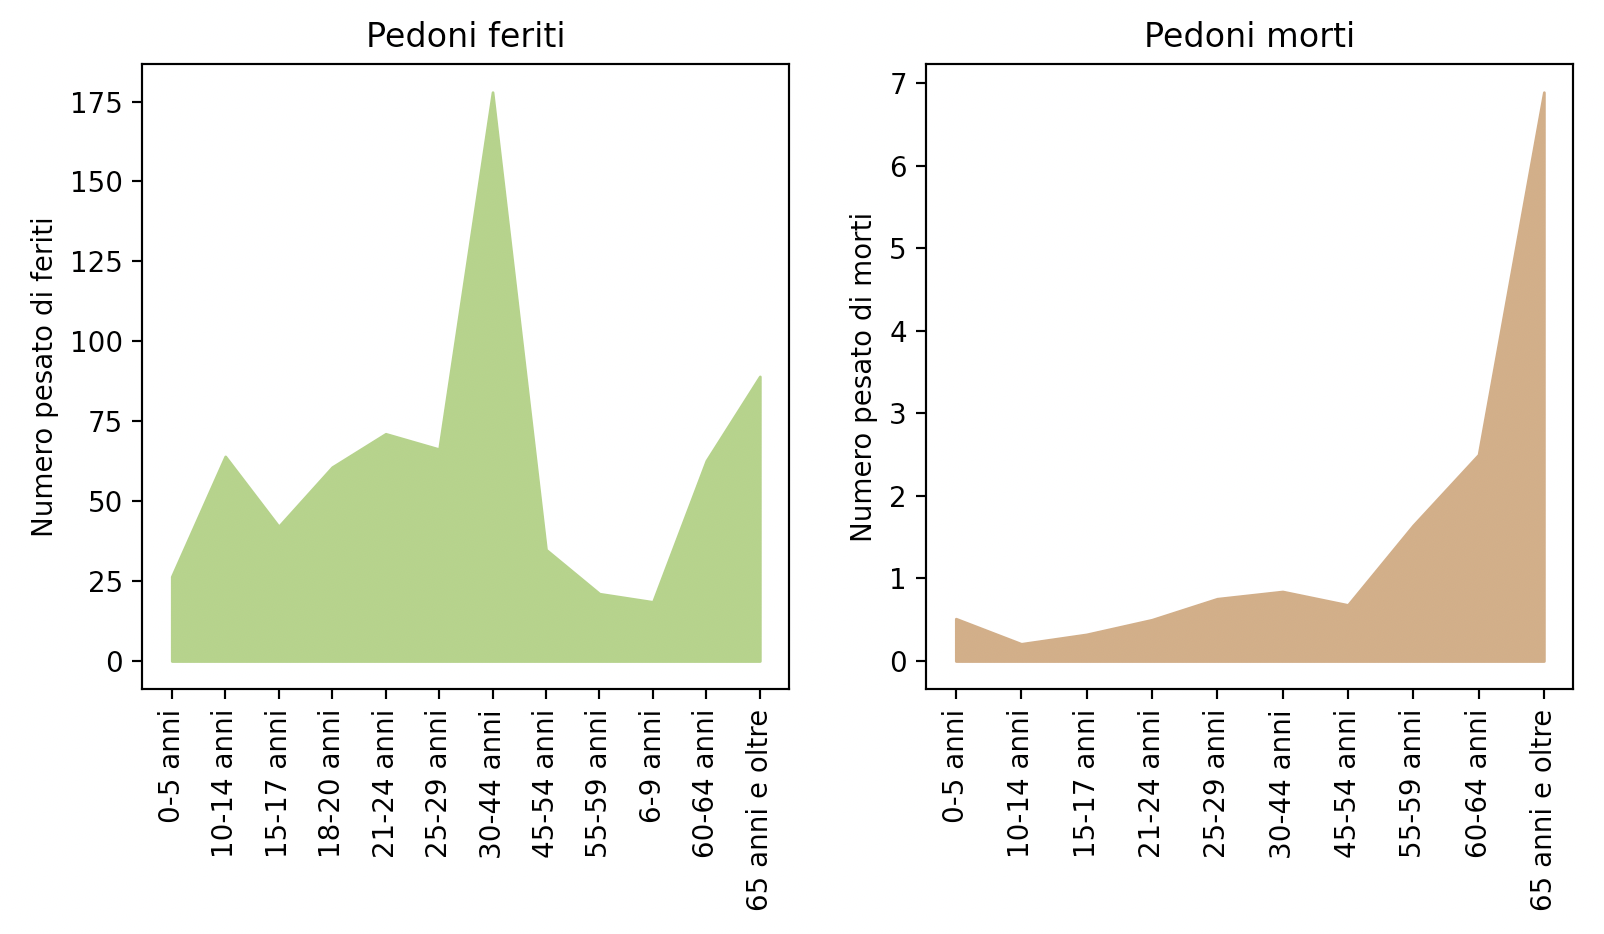
\includegraphics[width=\linewidth]{../src/incidenti/incidenti_senza_coords/pedoni/eta_pedoni_norm.png}
    \caption{Pedoni coinvolti in incidenti per et\'a}
    \label{fig:sesso_morti_feriti}
\end{figure}

La normalizzazione tiene conto che la fascia di et\'a '65 anni e oltre' vale venti anni.
%...

\begin{figure}[!ht]
    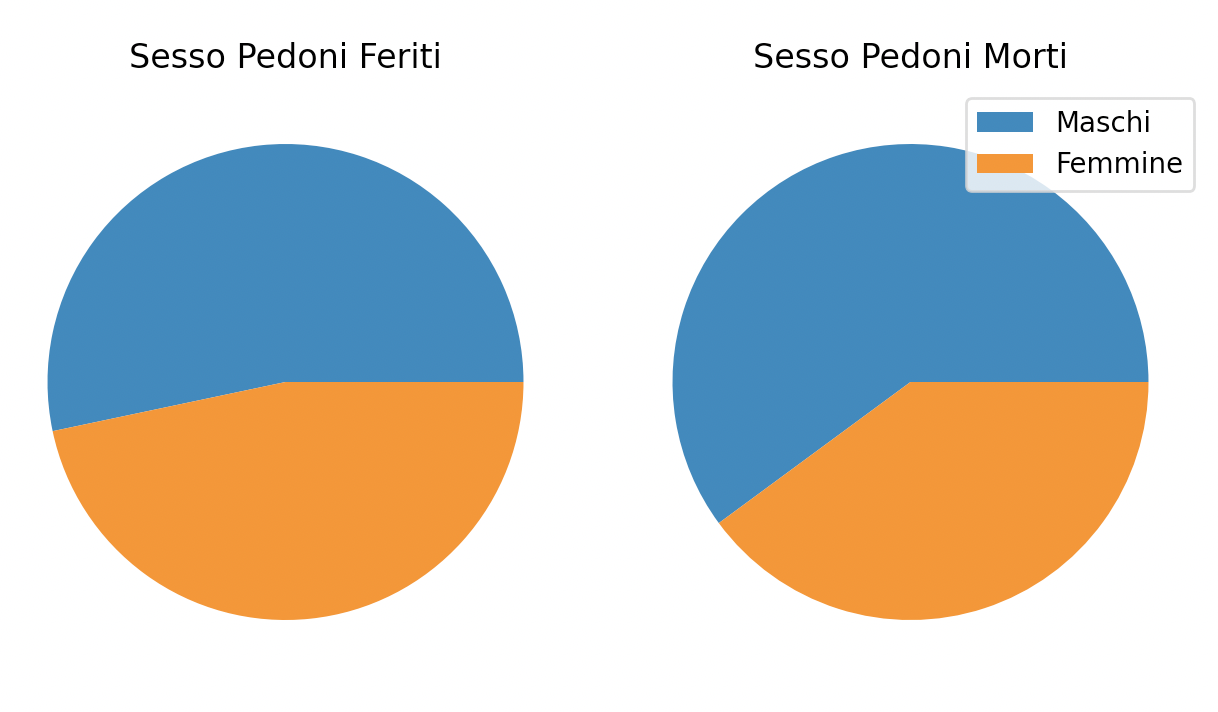
\includegraphics[width=\linewidth]{../src/incidenti/incidenti_senza_coords/pedoni/sesso_morti_feriti.png}
    \caption{Pedoni coinvolti in incidenti per genere}
    \label{fig:sesso_morti_feriti}
\end{figure}

Dati non sorprendenti\dots

%...




\newpage
\section{Dati ACI}

\newpage
\subsection{Quali sono le autostrade con pi\'u incidenti?}
\begin{figure}[!ht]
    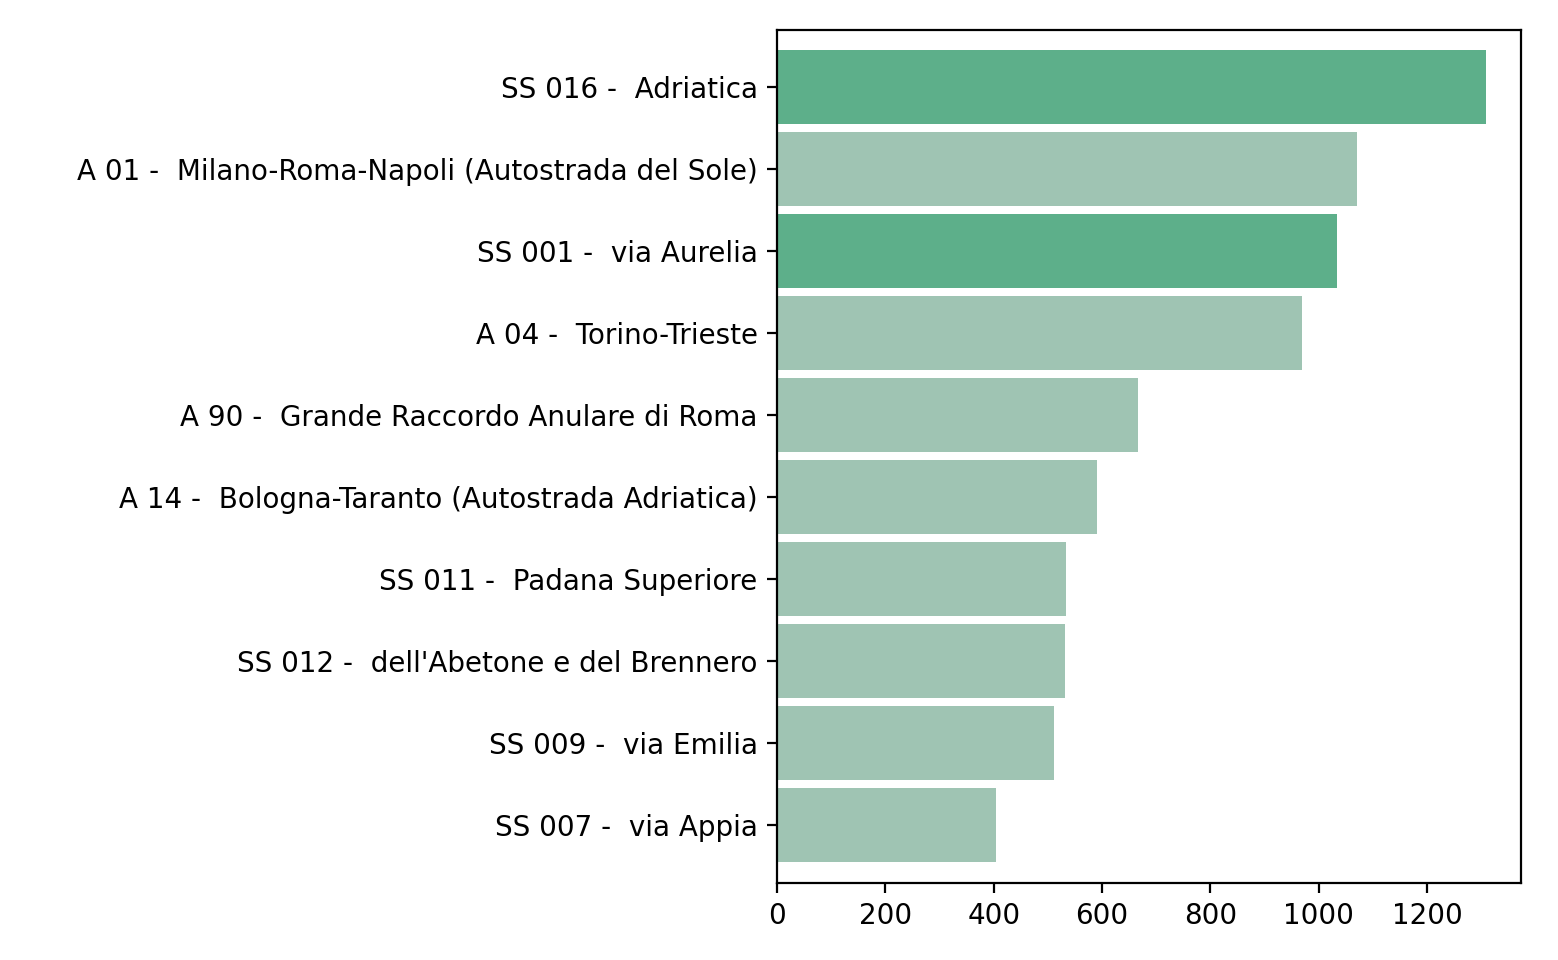
\includegraphics[width=\linewidth]{../src/incidenti/incidenti_aci/autostrade/autostrade.png}
    \caption{Autostrade con pi\'u incidenti nel 2018}
    \label{fig:incidenti_autostrade}
\end{figure}

Si pu\'o notare subito che le autostrade con pi\'u incidenti sono anche quelle pi\'u trafficate, come 
l'Autostrada del Sole e l'Adriatica.


%...

\newpage
\subsection{Autostrade pericolose a Milano?}

\begin{figure}[!ht]
    \includegraphics[width=\linewidth]{../src/incidenti/incidenti_aci/autostrade/incidenti_bubble_chart.png}
    \caption{Autostrade con pi\'u incidenti nel 2012}
    \label{fig:bubble_incidenti_milano}
\end{figure}



%...

\newpage
\subsection{In quali mesi avvengono pi\'u incidenti?}
\begin{figure}[!ht]
    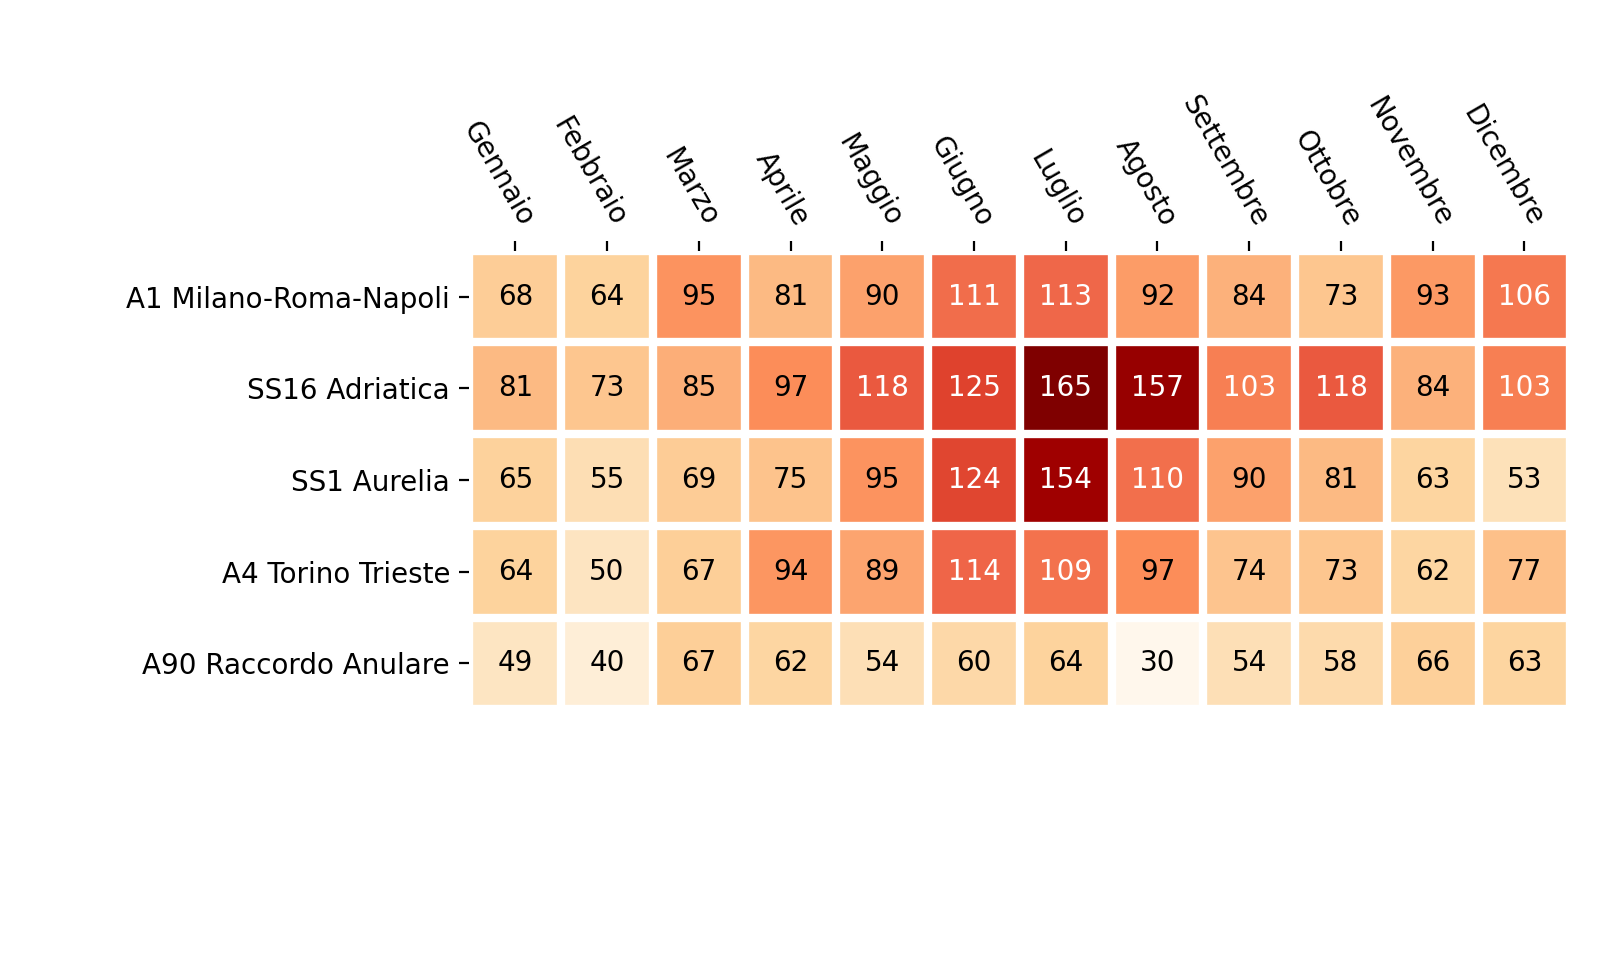
\includegraphics[width=\linewidth]{../src/incidenti/incidenti_aci/autostrade/mesi_autostrade.png}
    \caption{Incidenti per mese nel 2018}
    \label{fig:incidenti_per_mese}
\end{figure}

Le curve sono state normalizzate per bilanciare il volume di incidenti maggiori per 
l'autostrada Adriatica.
L'Adriatica e l'Aurelia, autostrade utilizzate molto durante i mesi caldi, hanno un picco di 
incidenti in Luglio e Agosto, mentre l'A1, ha picco pi\'u basso in Agosto, probabilmente 
perch\'e bilanciato dagli incidenti in inverno intorno a Milano.

% controllare se avvengono pi\'u incidenti in inverno intorno a milano
Infatti se si prendono solo i dati della A1 nella provincia di Milano, si nota 
che in Maggio e Settembre avvengono la maggior parte degli incidenti.
Invece sull'Adriatica prevalgono incidenti in Luglio e Agosto.
\begin{figure}[!ht]
    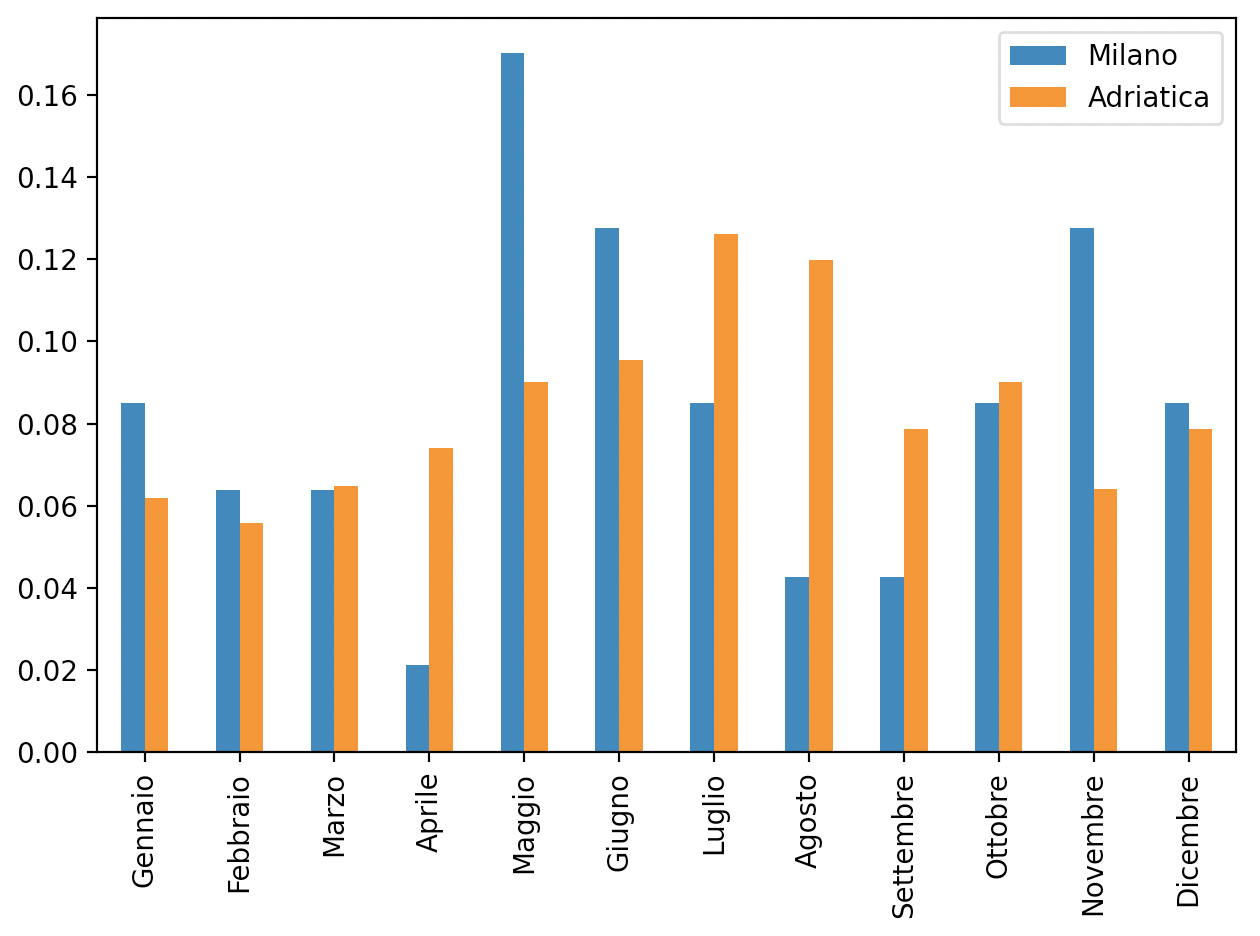
\includegraphics[width=\linewidth]{../src/incidenti/incidenti_aci/autostrade/milano_adriatica.png}
    \caption{Incidenti in provincia di Milano e sull'Adriatica}
    \label{fig:milano_adriatica}
\end{figure}

%...

\newpage%
\subsection{In Quali orari avvengono incidenti sulle autostrade?}
%TODO: orari di altri luoghi, ho fatto solo milano

\begin{figure}[!ht]
    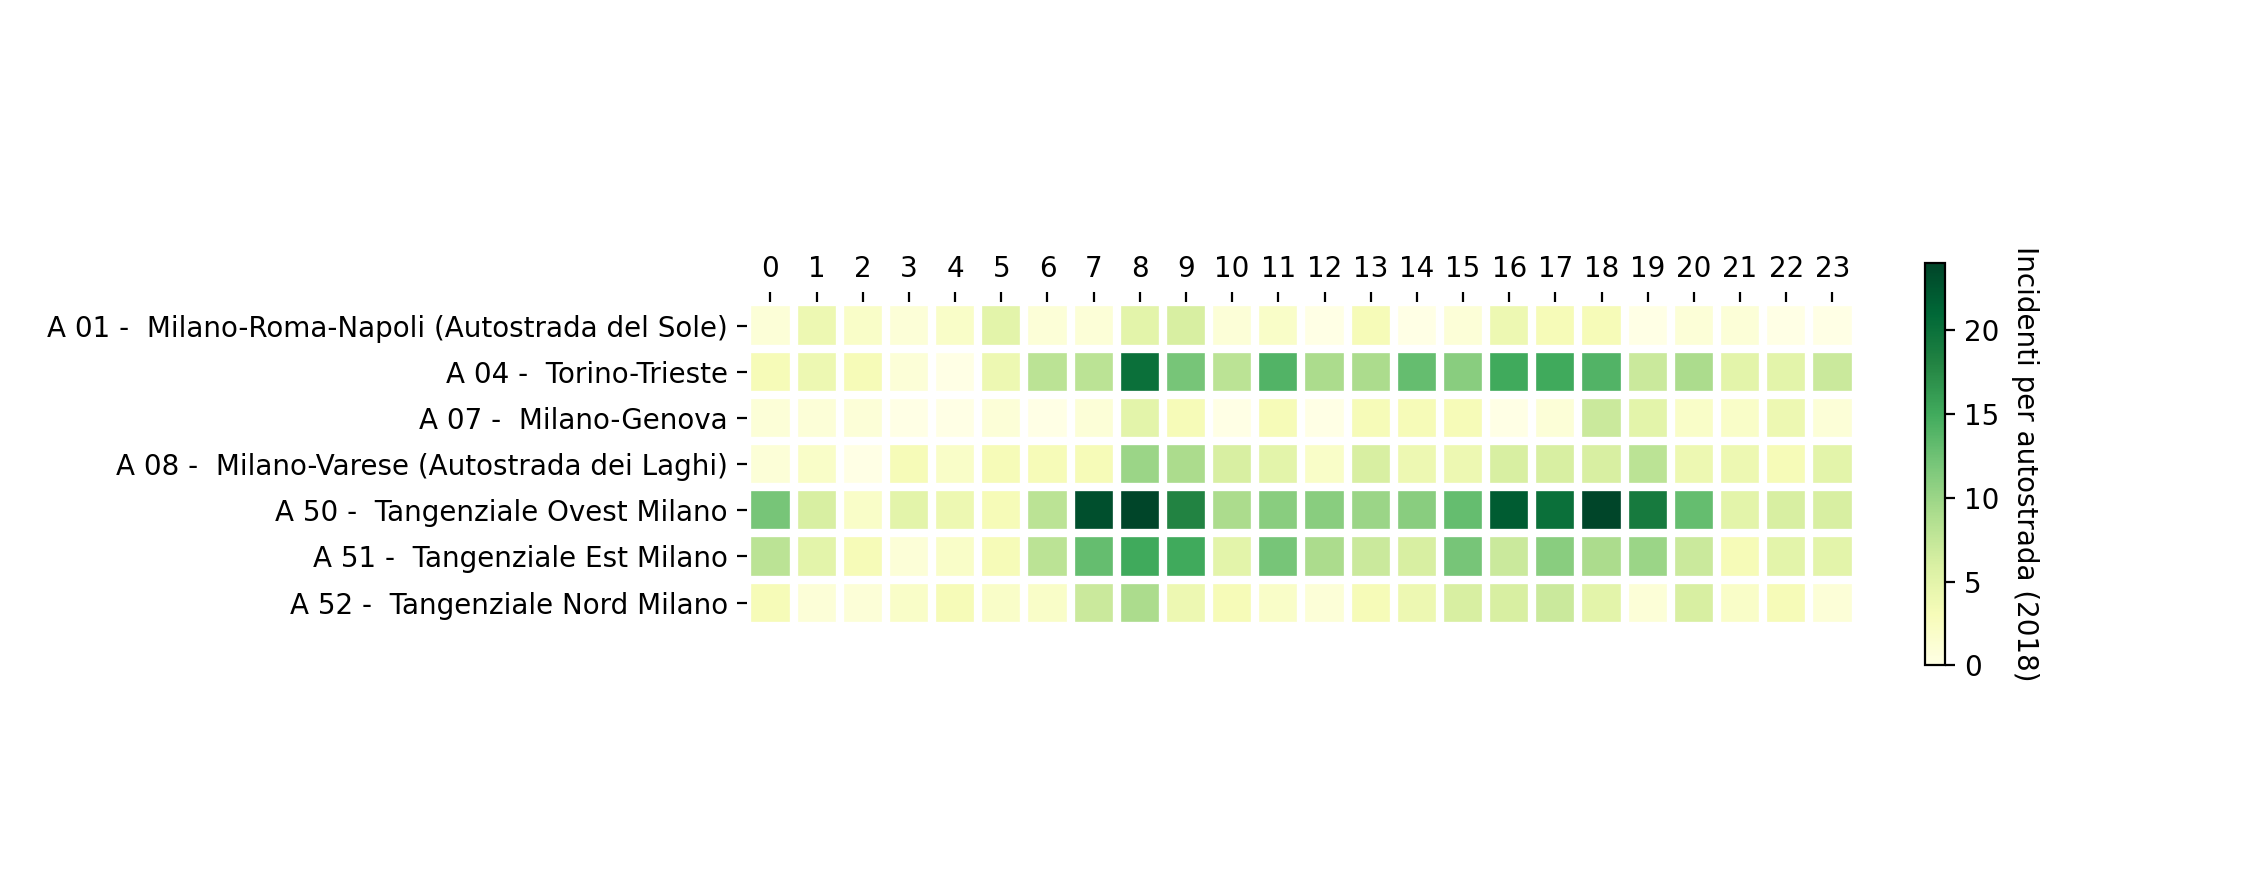
\includegraphics[width=\linewidth]{../src/incidenti/incidenti_aci/autostrade/tangenziali_autostrade.png}
    \caption{Incidenti nelle principali autostrade di Milano}
    \label{fig:milano_adriatica}
\end{figure}

\begin{figure}[!ht]
    \begin{subfigure}{\textwidth}
        \centering
    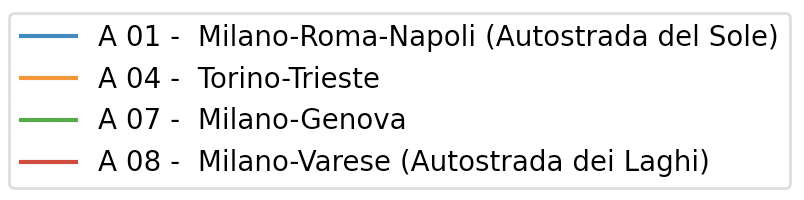
\includegraphics[width=0.6\linewidth]{../src/incidenti/incidenti_aci/autostrade/legenda_autostrade.png}
    \caption{Legenda Autostrade}
    \label{fig:legenda_autostrade}
    \end{subfigure}%
    \begin{subfigure}{\textwidth}
        \centering
    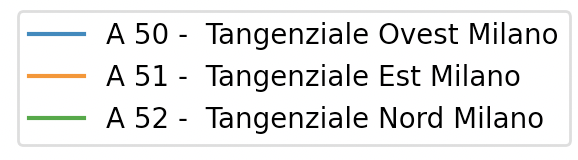
\includegraphics[width=0.5\linewidth]{../src/incidenti/incidenti_aci/autostrade/legenda_tangenziali.png}
    \caption{Legenda Tangenziali}
    \label{fig:legenda_tangenziali}
    \end{subfigure}
\end{figure}

Il grafo conferma per alcune autostrade i picchi di incidenti per il traffico durante orari 
di punta, in particolare \'e molto visibile per la Torino$-$Trieste e per la Tangenziale ovest.

%...



%%%%%%%%%%%%%%%%%%%%%%%%%%%%%%%%%%%%%%%%%%%%%%%%%%%%%%
\newpage
\chapter{Dati su Meteo}

\bibliographystyle{plain}
\bibliography{Biblio}
%\addcontentsline{toc}{chapter}{Bibliografia}

\end{document}
